%!TEX root = ../template.tex
%!TEX root = ../template.tex
%%%%%%%%%%%%%%%%%%%%%%%%%%%%%%%%%%%%%%%%%%%%%%%%%%%%%%%%%%%%%%%%%%%%
%% Desenvolvimento.tex
%% NOVA thesis document file
%%
%% Chapter with content
%%%%%%%%%%%%%%%%%%%%%%%%%%%%%%%%%%%%%%%%%%%%%%%%%%%%%%%%%%%%%%%%%%%%

\typeout{NT FILE Desenvolvimento.tex}%

\prependtographicspath{{Chapters/Figures/}}

% epigraph configuration
\epigraphfontsize{\small\itshape}
\setlength\epigraphwidth{12.5cm}
\setlength\epigraphrule{0pt}

\chapter{Mapeamento dos Exames}
\label{cha:mapeamento_dos_exames}

%Este capítulo irá descrever como se procedeu ao mapeamento dos exames mais frequentes, que considerações foram tidas, que simplificações apresentam e o resultado final desta fase.\\

O processo de mapeamento dos exames começou com a decisão sobre quais incluir no estudo. Nem todos os exames foram considerados devido à baixa frequência com que estes ocorrem e a consequente falta de dados em relação à duração das suas atividades. Desta forma, apenas foram mapeados aqueles que ocorrem pelos menos mensalmente.\\
De seguida, foi necessário definir os recursos-tipo existentes no sistema, estes podem ser divididos em recursos humanos e em recursos físicos. A Figura~\ref{tab:cap_rec} apresenta cada recurso-tipo, a correspondente abreviatura e quantidade.

\begin{table}[H]
\caption{Capacidade dos vários recursos,}
\label{tab:cap_rec}
\begin{tabular}{c|l|l|l}
Tipo                                                                                           & Nome do Recurso                                  & Abreviatura & Quantidade \\ \hline
\multirow{5}{*}{\shortstack{Recursos\\Humano}}                                                 & Técnicos Auxiliares de Saúde                     & TAS         & 4          \\
                                                                                               & Enfermeiros                                      & ENF         & 4          \\
                                                                                               & Técnicos Superiores de Diagnóstico e Terapêutica & TSDT        & 4          \\
                                                                                               & Médicos Especialistas                            & ME          & 2          \\
                                                                                               & Médicos Cardiologistas                           & MC          & 1          \\ \hline
\multirow{10}{*}{\shortstack{Recursos\\Físico}}                                                & Gabinete Médico                                  & GM          & 2          \\
                                                                                               & Sala de Espera                                   & SE          & 4          \\
                                                                                               & Sala de Espera de Crianças                       & SEC         & 3          \\
                                                                                               & Sala de Espera para Doentes Acamados             & SC          & 2          \\
                                                                                               & Sala Polivalente                                 & SP          & 1          \\
                                                                                               & Sala Enfermagem 1                                & SE1         & 1          \\
                                                                                               & Sala Enfermagem 2                                & SE2         & 3          \\
                                                                                               & Sala Enfermagem 1                                & SE3         & 3          \\
                                                                                               & Sala Câmara Gama                                 & SCG         & 1          \\
                                                                                               & Sala Tomografo                                   & ST          & 1         
\end{tabular}
\end{table}

Cada recurso-tipo tem uma quantidade de recursos disponíveis. Para os recursos humanos corresponde ao número de profissionais em cada grupo existentes no departamento e para os recursos físicos corresponde à lotação de pacientes que podem suportar. Iremos considerar que existe portanto uma capacidade máxima para cada recurso-tipo. Admite-se que cada recurso atribuído a uma tarefa será utilizado durante a sua duração total.\\

Considerou-se ainda a possibilidade de ter a capacidade dos recursos variável com o tempo, de forma a modelar os diferentes turnos e os períodos onde existe mudança entre estes. Com mais discussão decidiu-se que as diferenças existente ao longo do dia relativamente à capacidade de cada recurso é mínimo, mas será fácil incluir este aspeto num estudo futuro.\\

Existem recursos-tipo que podem ser equiparados a outros em certas atividades. A SP e a SE1 podem ser tidas como equivalentes em certas atividades. Por isso foi necessário criar recursos-tipo fictícios. Para o exemplo anterior, foi criado o recurso-tipo SP ou SE1, sempre que uma destas salas é explicitamente necessária, a sua utilização é representadas no recurso-tipo correspondente e no recurso-tipo fictício, caso seja indiferente a sala necessárias a utilização apenas é representada no recurso-tipo fictício.\\

A SE2 e a SE3 podem também ser tidas como equiparadas, mas quando a SE2 é explicitamente necessária toda ela é ocupada por uma pessoa, efetivamente diminuindo a sua capacidade de três para uma pessoa, ocorrendo em algumas atividades do exame cintigrafia pulmonar de ventilação/inalação + perfusão. O recurso fictício SE2 ou SE3 continua a ter uma capacidade de seis pessoa. Ambos os casos apresentam-se na Tabela~\ref{tab:cap_RFic}, onde se observa a capacidade efetiva destes recursos.\\
\begin{table}[H]
\centering
\caption{Capacidade dos recursos-tipo fictícios}
\label{tab:cap_RFic}
\begin{tabular}{l|llllllllll}
Recursos-tipo fictícios & SP & SE1 & SP ou SE1 & SE2 & SE2 ou SE3\\ \hline
Quantidade              & 1  & 1   & 2         & 1   & 6
\end{tabular}
\end{table}

Num passo seguinte, cada exame foi decomposto nas suas atividades. Considerou-se que uma nova atividade deve começar quando existe uma mudança dos recursos necessários. Foram então realizadas entrevistas de forma a realizar a decomposição dos exames. No seguimento das entrevistas as atividades foram validadas pelos vários grupos profissionais. Rapidamente, SE identificou a necessidade de diferenciar o mapeamento entre pacientes com mobilidade autónoma, aqueles com mobilidade condicionada, e crianças existindo diferenças nos recursos necessários e na duração de cada atividade.\\
Seguidamente, as duração de cada atividade foram recolhidas utilizando folhas de registo provenientes do mapeamento realizado. A duração média de cada atividade foi obtida através da hora de início e de fim de cada atividade registadas pelos profissionais. Será de salientar que mesmo sendo este um problema de \textit{No-Wait}, esta restrição nem sempre foi verificado nas folhas de registo.\\

Em certas atividades considera-se que a permanência de um recurso durante a sua totalidade como uma simplificação do problema. Podemos utilizar como exemplo a atribuição de um TAS ao tempo de espera decorrido dentro do departamento por cada paciente, contudo não foi possível definir explicitamente quando é que estes recursos seriam necessários, sendo esta uma fonte de variabilidade do sistema, impossibilitando a decomposição da atividade.\\ 
Todas as folhas de registo e respetivos dados estão em anexo a esta dissertação.\\

Através da Figura~\ref{fig:full_exams} podemos observar qual a utilização dos recursos provenientes de uma agenda, em conjunto com a Figura~\ref{fig:one_exam_each} torna-se possível identificar quais exames podem ser inseridos sem ter grande impacto sobre o valor de \textit{makespan}.
\begin{figure}[h]
	\centering
	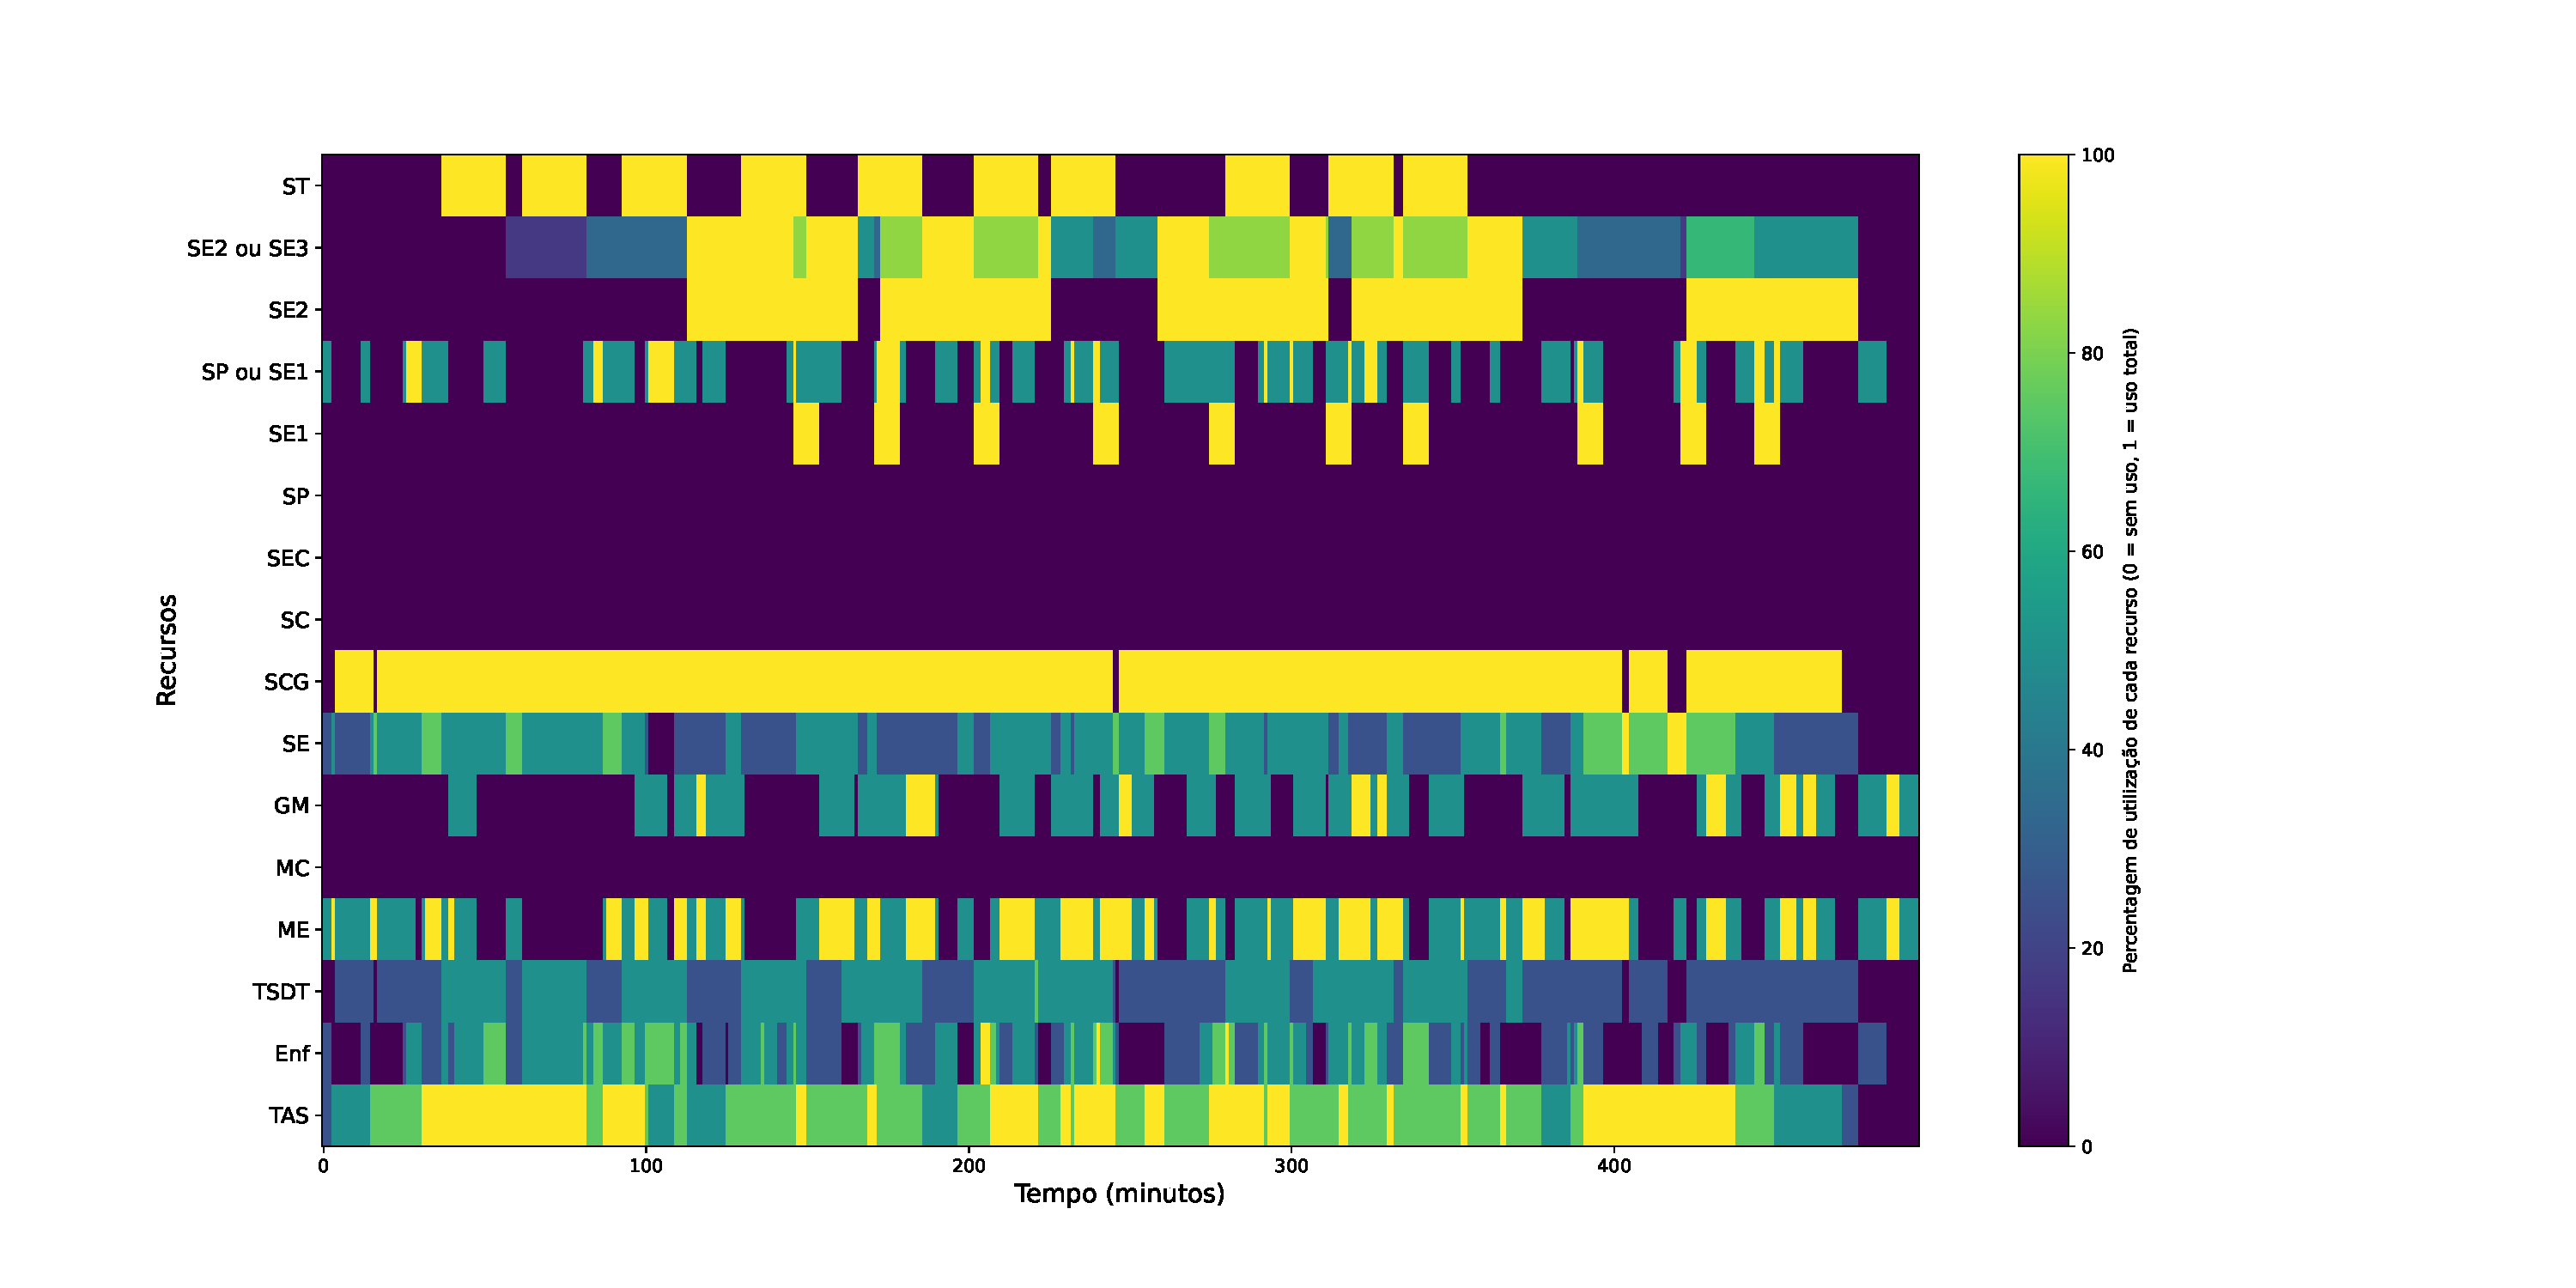
\includegraphics[clip, trim=3cm 1cm 9cm 2.5cm, width = 0.75\textwidth]{full_exams}
	\caption{Utilização de recursos-tipo de uma agenda}
	\label{fig:full_exams}
\end{figure}

\begin{figure}[h]
	\centering
	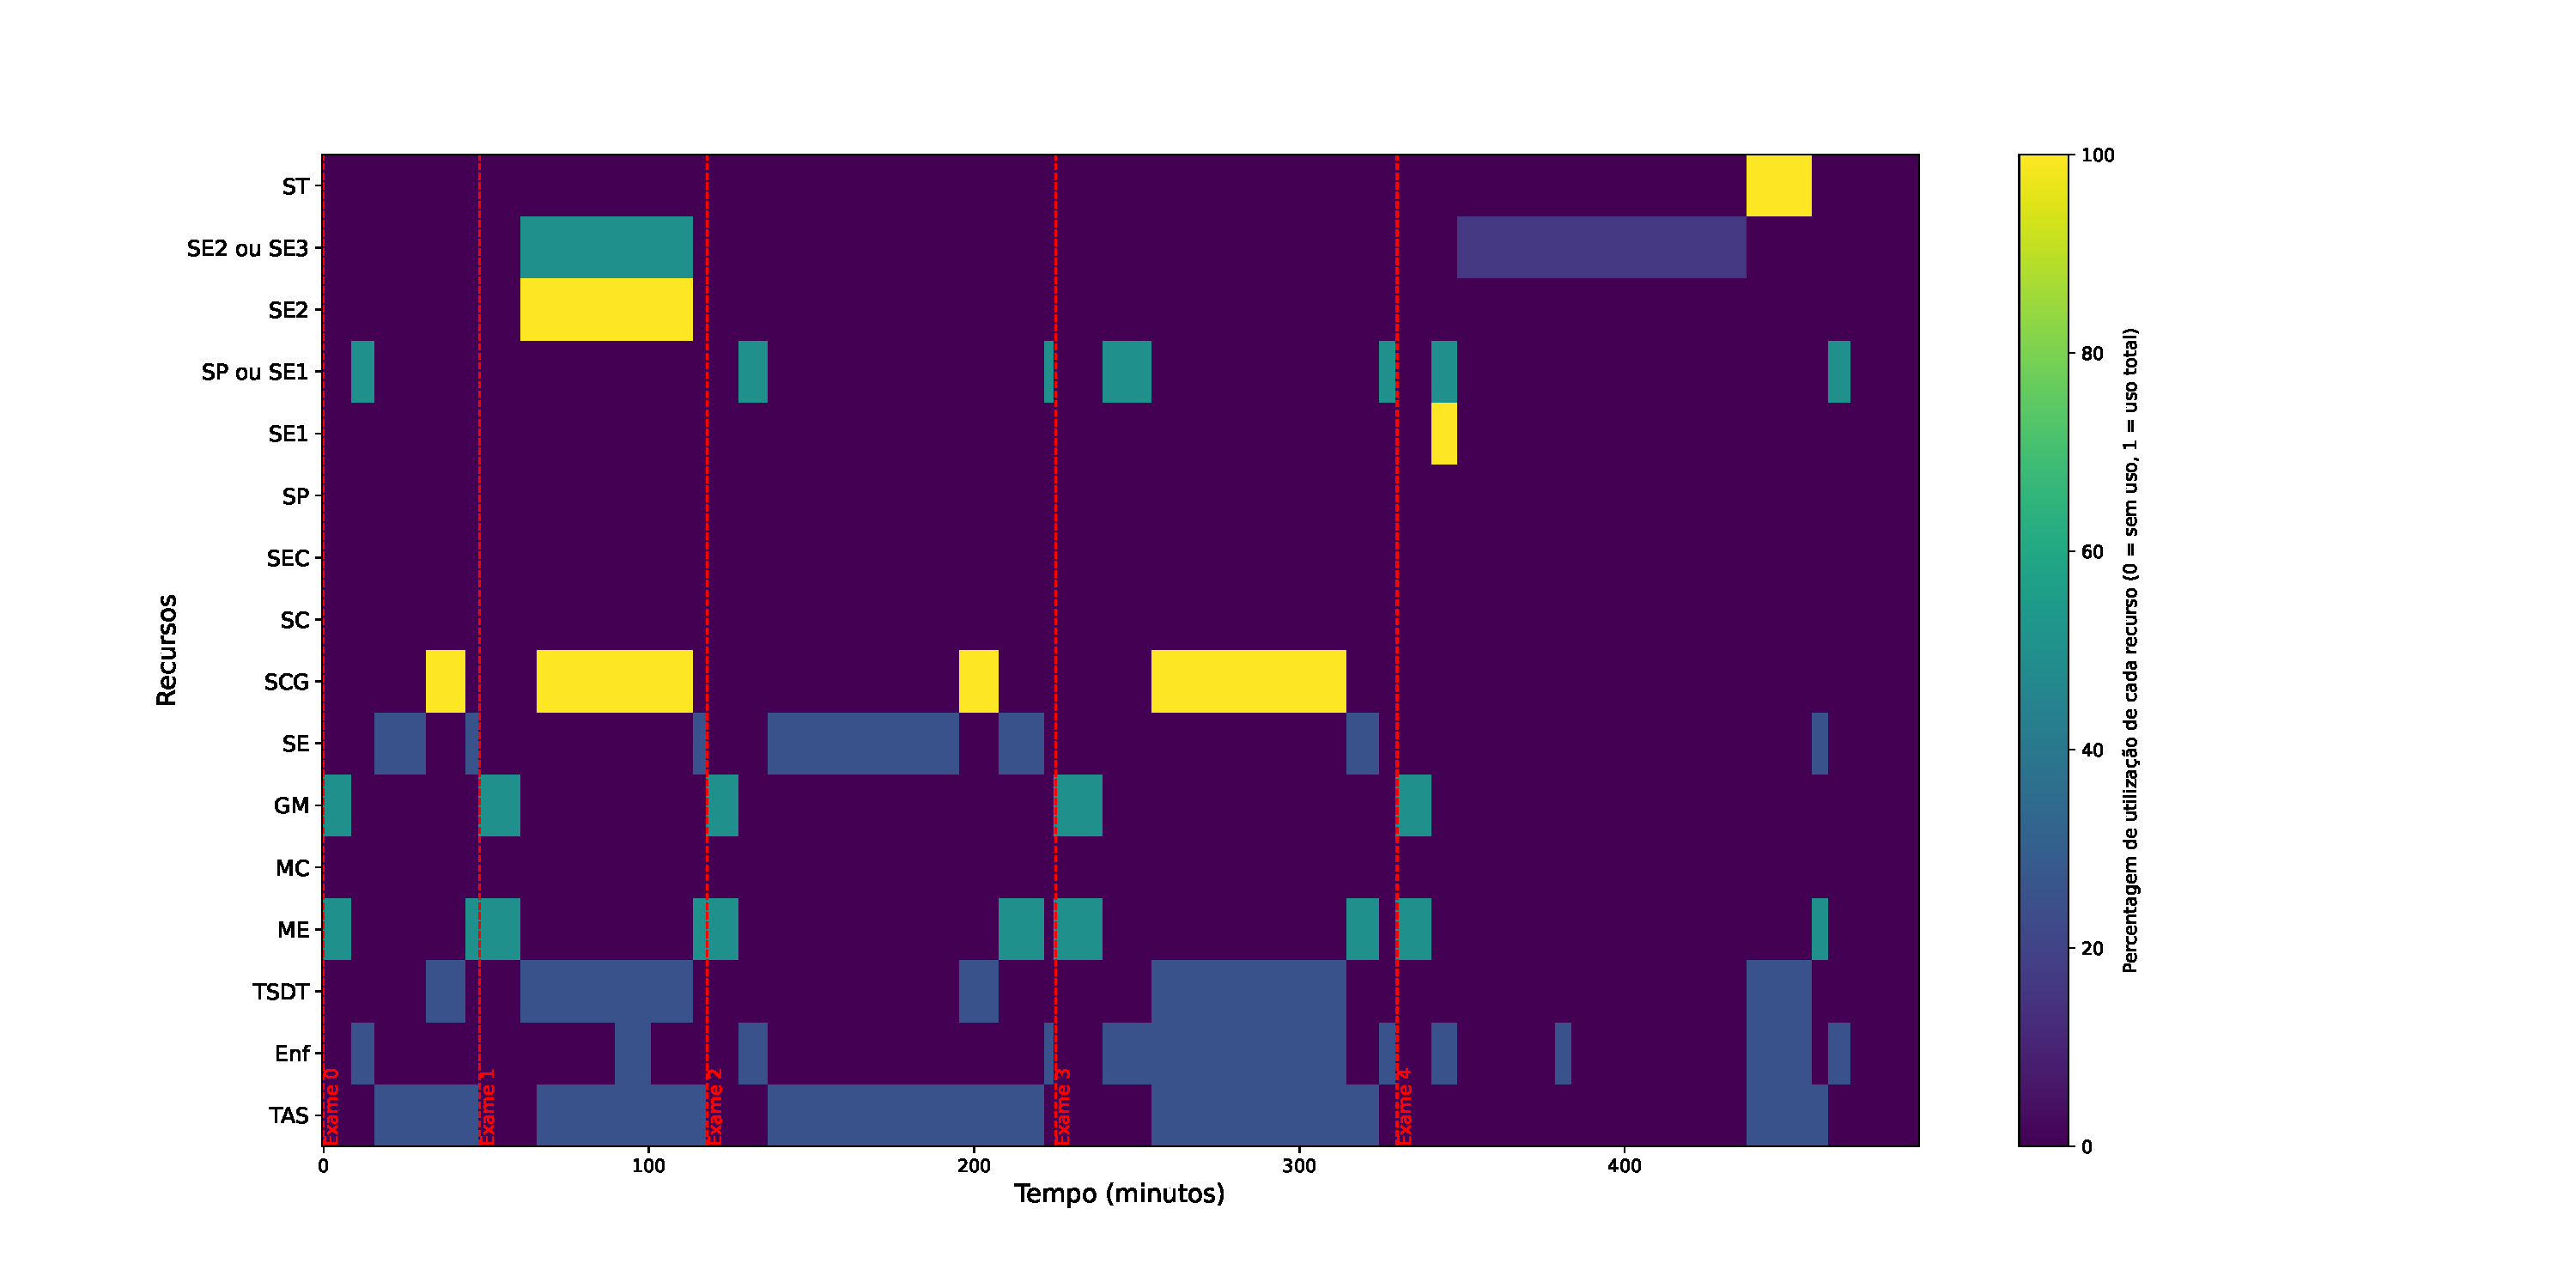
\includegraphics[clip, trim=3cm 1cm 9cm 2.5cm, width = 0.75\textwidth]{one_exam_each}
	\caption{Utilização de recursos-tipo repartidos por exames}
	\label{fig:one_exam_each}
\end{figure}

Visualmente identifica-se que SCG é o principal recurso limitante ao estar quase toda a sua duração a ser utilizado na totalidade. Outros recursos que são também limitantes são ST e SE2, estes são utilizados por menos exames, contudo os exames que os necessitam tendem a ocorrer em grandes números. Recursos como SP, SEC, SC, e MC só são necessários em casos específicos e por isso não tendem a apresentar utilização alta.\\

\chapter{Desenvolvimento dos Modelos}
\label{cha:desenvolvimentos_dos_modelos}

Neste capítulo, dois problemas devem ser resolvidos, tendo para isso sido desenvolvidos vários modelos. No primeiro problema existem recursos e exames fixos, sendo o objetivo minimizar o tempo entre o começo e o fim de todos os exames, chamado de \textit{makespan}. O segundo problema tem recursos e tempo fixos, sendo o objetivo maximizar o número de exames a realizar, utilizando um somatório simples ou ponderado.

\section{Problema de \textit{Makespan}}

Este problema utiliza o exemplo de uma segunda-feira típica em termos de exames realizados. Ocorrendo 3 cintigrafia tiroideia, 5 cintigrafia pulmonar de ventilação/inalação + perfusão, 10 cintigrafia miocárdica de perfusão em repouso, 1 cintigrafia das glândulas salivares, 10 PET - estudo corpo inteiro com FDG.\\

A próxima formulação segue sensivelmente a formulação de Kondili et al.~\cite{kondiliGeneralAlgorithmShortterm1993}, com as modificações necessárias para obedecer às extensões e restrições propostas, continuando a ser uma formulação indexada no tempo, chamá-la-emos de \textit{MILP-trad}:\\

Conjuntos:\\
O conjunto de trabalhos $I, i \in I := (1, \ldots, n)$ \\
O conjunto de operações $K, k \in K := (1, \ldots, K_{\max})$ \\
O conjunto de recursos-tipo $R, p \in R := (1, \ldots, R_{\max})$ \\
O conjunto de instantes de tempo $T, t \in T := (1, \ldots, T_{\max})$ \\

Parâmetros:\\
$\rho_{i,k}$ é o tempo de processamento da operação $k$ do trabalho $i$ \\
$r_{i,p,k}$ é quantidade $p$ necessária para realizar a operação $k$ do trabalho $i$ \\
$C_{p}$ é a capacidade do recurso $p$ \\

Variáveis de Decisão: \\
$X_{t,i,k}$ é uma variável binária com valor 1 se a operação $k$ do trabalho $i$ ocorrer durante o instante $t$, caso contrário tem valor 0 \\
$Z_{t,i,k}$ é uma variável binária com valor 1 se a operação $k$ do trabalho $i$ começar no instante $t$, caso contrário tem valor 0 \\
$S_{i,k}$ é uma variável inteira que representa o valor de começo da operação $k$ do trabalho $i$ \\
$F_{i,k}$ é uma variável inteira que representa o valor de fim da operação $k$ do trabalho $i$ \\
$C_{\max}$ é uma variável inteira que representa o \textit{makespan} \\

Função Objetivo:
\begin{align}
\min C_{\max} \label{eq:1}
\end{align}

Sujeito a:
\begin{align}
&F_{i,K_{\max}} \leq C_{\max} \quad \forall i \label{eq:2} \\
&\sum_{t}Z_{t,i,k} = 1 \quad \forall i,k \label{eq:3} \\
&\sum_{t}X_{t,i,k} = \rho_{i,k} \quad \forall i,k \label{eq:4} \\
&\sum^{t+\rho_{i,k}}_{t^{'}=t}X_{t^{'},i,k} \geq \rho_{i,k}Z_{t,i,k} \quad \forall i,k,t=1, \ldots,T-\rho_{i,k} \label{eq:5} \\
&S_{i,k} = \sum_{t}tZ_{t,i,k} \quad \forall i,k \label{eq:6} \\
&S_{i,k+1} = F_{i,k} \quad \forall i,k \label{eq:7} \\
&F_{i,k} - S_{i,k} = \rho_{i,k} \quad \forall i,k \label{eq:8} \\
&\sum_{i}\sum_{k}r_{i,p,k}X_{t,i,k} \leq C_{p} \quad \forall t,p \label{eq:9} 
\end{align}
A função objetivo (~\ref{eq:1}) minimiza o \textit{makespan} dos trabalho, ou seja, o tempo entre o início do primeiro exame, e o fim do último.\\
A restrição (~\ref{eq:2}) garante que todos os trabalho acabam antes ou no instante do \textit{makespan}, auxiliando a função objetivo.\\
A restrição (~\ref{eq:3}) garante que só existe um instante em que a operação $k$ do trabalho $i$ é atribuído.\\
A restrição (~\ref{eq:4}) garante, que para a operação $k$ do trabalho $i$, o somatório de $X_{t,i,k}$ sobre $t$ tem o valor da duração $\rho_{i,k}$. \\
A restrição (~\ref{eq:5}) garante a concordância do posicionamento sobre $t$ entre $X_{t,i,k}$ e $Z_{t,i,k}$. \\
A restrição (~\ref{eq:6}) garante a coerência do momento de início da tarefa $k$.\\
A restrição (~\ref{eq:7}) garante que, para o trabalho $i$, a operação $k+1$ começa quando a operação $k$ acaba, verificando a restrição de \textit{No-Wait}. \\
A restrição (~\ref{eq:8}) garante que a duração da operação $k$ para o trabalho $i$ é de $\rho_{i,k}$.\\
A restrição (~\ref{eq:9}) garante que não existe a sobre-utilização do recursos $p$ durante o instante $t$, verificando as extensões \textit{Multi-Resource} e \textit{Flexible}.\\

Por outro lado, é possível formular modelos mais eficientes do que o clássico. A formulação aqui sugerida, \textit{MILP-$\delta$}, tira partido do facto da restrição \textit{No-Wait} criar um padrão de utilização de recursos, qualquer que seja o instante $t$ onde este se insere. Desta forma, não é necessário explicitamente formular restrições que garantem \textit{No-Wait}.\\

Conjuntos:\\
O conjunto de trabalhos $I, i \in I := (1, \ldots, n)$ \\
O conjunto de recursos-tipo $R, p \in R := (1, \ldots, R_{\max})$ \\
O conjunto de instantes de tempo $T, t \in T := (1, \ldots, T_{\max})$ \\

Parâmetros:\\
$\rho_{i}$ é duração do trabalho $i$ \\
$\delta_{i}(u,p)$ é a quantidade de recursos do tipo $p$ necessários a um offset de $u$ instantes de tempo no trabalho $i$\\
$C_{p}$ é a capacidade do recurso $p$ \\

Variáveis de Decisão: \\
$Z_{t,i}$ é uma variável binária com valor 1 se o trabalho $i$ começar no instante $t$, caso contrário tem valor 0 \\
$F_{i}$ é uma variável inteira que representa o valor de fim do trabalho $i$ \\
$C_{\max}$ é uma variável inteira que representa o \textit{makespan} \\

Função Objetivo:
\begin{align}
\min C_{\max} \label{eq:10}
\end{align}

Sujeito a:
\begin{align}
&F_{i} \leq C_{\max} \quad \forall i \label{eq:11} \\
&\sum^{T_{\max}-\rho_{i}+1}_{t=0}Z_{t,i} = 1 \quad \forall i \label{eq:12} \\
&\sum^{T_{\max}-\rho_{i}+1}_{t=0}Z_{t,i}*(t+\rho_{i}) = F_{i} \quad \forall i \label{eq:13} \\
&\sum_{i}\sum^{\min(t, T_{\max}-\rho_{i})}_{\tau=\max(0, t-\rho_{i}+1)}\delta_{i}(t-\tau,p)Z_{\tau,i} \leq C_{p} \quad \forall t,p \label{eq:14}
\end{align}
A função objetivo (~\ref{eq:10}) minimiza o \textit{makespan} dos trabalhos.\\
A restrição (~\ref{eq:11}) garante que todos os exames acabam antes ou no instante do \textit{makespan}, auxiliando a função objetivo.\\
A restrição (~\ref{eq:12}) garante que só existe um instante de começo do trabalho $i$.\\
A restrição (~\ref{eq:13}) faz a ligação entre as variáveis $Z_{t,i}$ e $F_{i}$.\\
A restrição (~\ref{eq:14}) garante que não há sobre-utilização de recursos, ao verificar. para cada instante $t$, quais trabalhos estão a ser executados e em que fase este se encontra, garantindo que em cada instante não há sobre-utilização de recursos.\\

Para ambas das formulações apresentadas, o tamanho do conjunto de instantes de tempo, $T$, tem impacto no número de variáveis e restrições. Será por isso importante encontrar o menor valor de $T_{\max}$ possível mas que seja maior que \textit{makespan}, a isto tipicamente chama-se de \textit{upper-bound}.\\ 

De seguida, foram desenvolvidos três modelos, utilizando \textit{SA}, com duas codificações de solução diferentes. Os dois primeiros modelos utilizam uma codificação que representa o instante de início de cada trabalho. O outro modelo utiliza a sequência de escalonamento de cada trabalho como solução.\\

\textit{SA} foi a meta-heurística escolhida devido a alguns fatores. Devido ao algoritmo de Metropolis, esta meta-heurística é capaz de escapar a mínimos locais através da aceitação de soluções que pioram a função objetivo. Ao mesmo tempo, com a escolha correta dos níveis das variáveis do algoritmo existe garantia de se alcançar a solução ótima~\cite{delahayeSimulatedAnnealingBasics2019}.\\

\subsection{Modelo 1}

Este modelo é definido pelo o facto de não existir a garantia da viabilidade de cada solução. Por isso é necessário criar uma função objetivo diferente das restante, esta será dada por:
$$f(s) = C_{\max} + P \sum_{t=start}^{end-1}\sum_{p}v(t,p)$$

Onde $C_{\max}$ é \textit{makespan}, $P$ a punição relativamente à sobre-utilização de recursos (sendo esta uma variável a estudar). Esta sobre-utilização é dada pelo somatório dos recursos e instantes de tempo, $v(t,p)$ que por sua vez é dado por:
$$
v(t,p)=
\begin{cases}
	1 & \text{se } u(t,p)>C_{p}\\
	0 & \text{caso contrário}
\end{cases}
$$

Temos que $u(t,p)$ é a utilização de cada recurso $p$ em cada instante $t$, $C_{p}$ será a capacidade máxima de cada recurso, tornando-se assim uma variável binária para cada recurso e instante. Poderia ter-se considerado uma definição diferente de $v(t,p)$:
$$
v(t,p)=
\begin{cases}
	u(t,p)-C_{p} & \text{se } u(t,p)>C_{p}\\
	0            & \text{caso contrário}
\end{cases}
$$

Apesar de corresponder melhor à verdadeira sobre-utilização de recursos, ao diferenciar a quantidade, esta formulação apresenta piores resultados.\\

Será de salientar como $C_{\max}$ é calculado, dado que existem duas formas semelhantes para tal. A Figura~\ref{fig:0_makespan} apresenta a primeira forma, temos que \textit{makespan} é dado pelo máximo do término de cada trabalho, \textit{fim}. Por sua vez, a Figura~\ref{fig:start_end} apresenta a alternativa para o cálculo de \textit{makespan}, ao considerar que este valor é obtido pela diferença entre o valor máximo de término de cada trabalho e o valor mínimo de início de cada trabalho, \textit{fim-ini}. Ambas as figuras representam três soluções distintas, com o segmento a vermelho a demonstrar o aparente valor de \textit{makespan}. Utilizou-se a segunda forma para calcular \textit{makespan} porque esta não pune uma solução só por esta não começar no instante 0.\\
\begin{figure}[H]
	\centering
	\begin{subfigure}{0.49\textwidth}
	\centering
		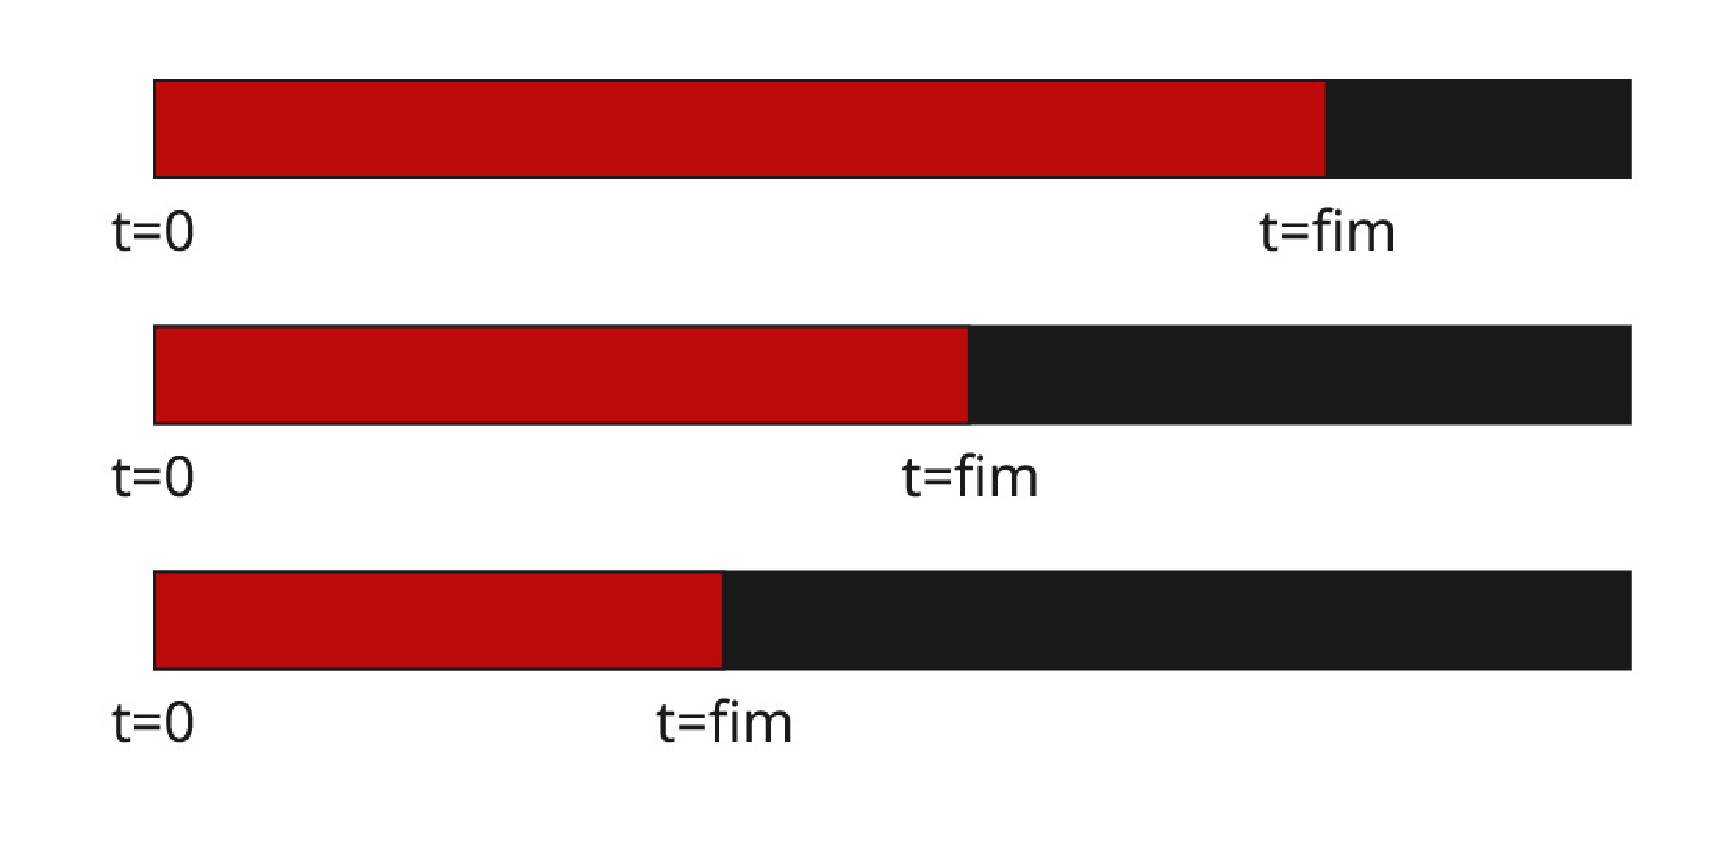
\includegraphics[width = \textwidth]{0_makespan}
		\caption{\textit{Makespan} definido por \textit{fim}}
		\label{fig:0_makespan}
	\end{subfigure}
	\begin{subfigure}{0.49\textwidth}
	\centering
		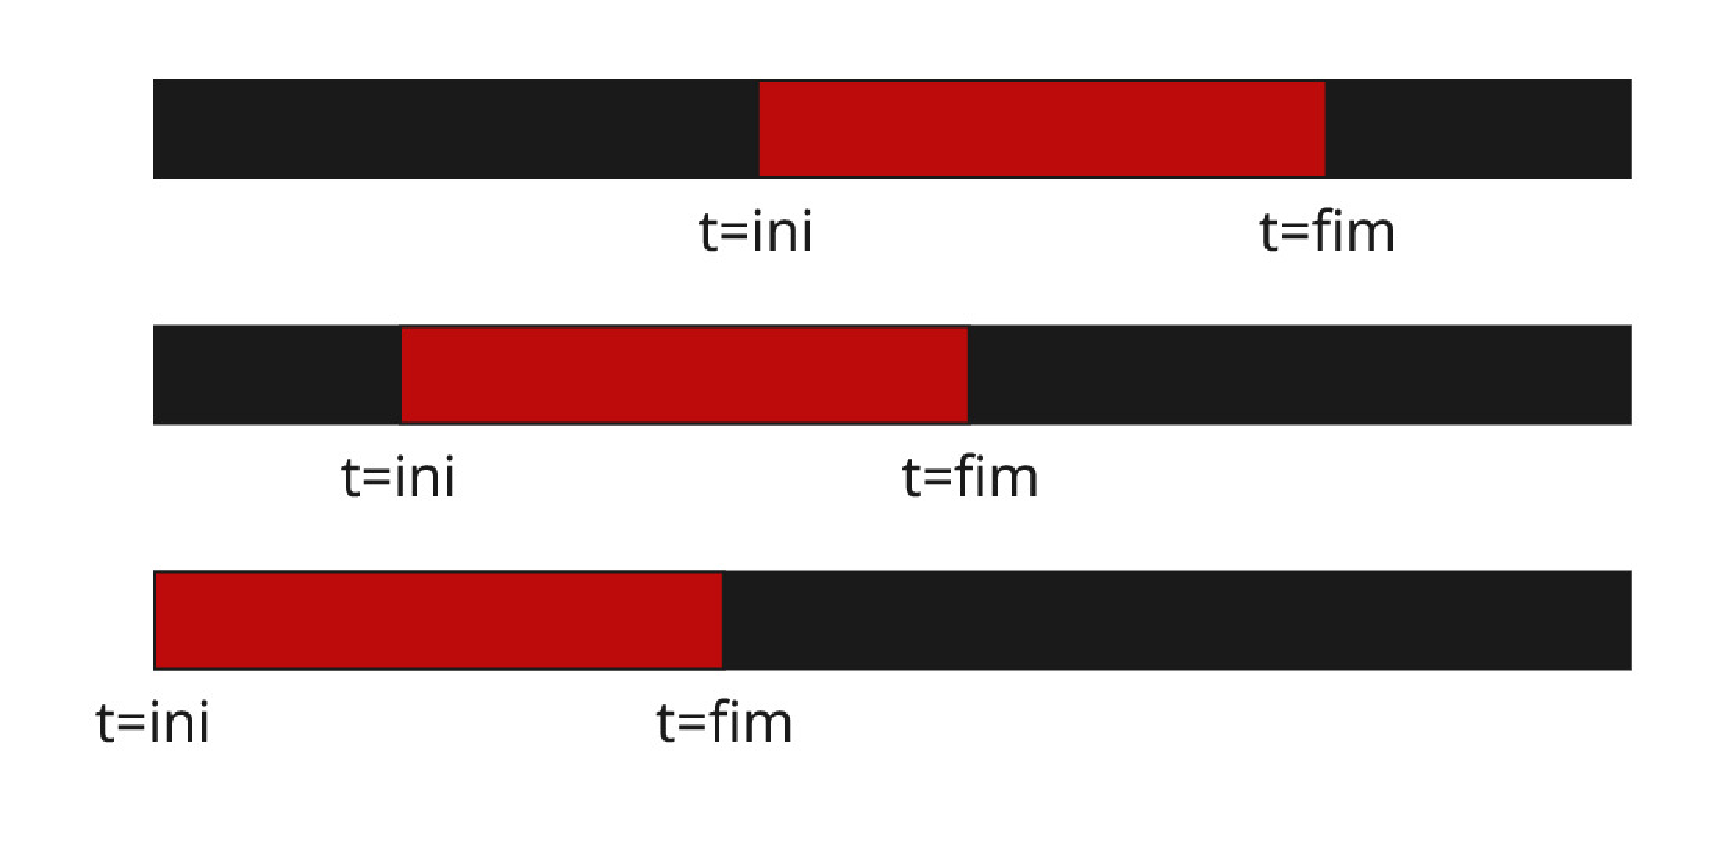
\includegraphics[width = \textwidth]{start_end}
		\caption{\textit{Makespan} definido por \textit{fim-ini}}
		\label{fig:start_end}
	\end{subfigure}
	\caption{Impacto das duas formas de calcular \textit{makespan}.}
	\label{fig:dif_makespan}
\end{figure}

Para este modelo, a solução $s$ é dada pelo instante $t$ em que começa cada trabalho $i$. Por sua vez, a vizinhança de $s$, $S_{s}$, é definida pelo trabalho a reagendar e quando este deve começar. Ambos estes valores são obtidos aleatoriamente, contudo $t$ poderá ser obtido através de uma distribuição uniforme U(0, \textit{makespan}-d), ou U(\textit{ini}, \textit{fim}-d), sendo d a duração do tempo necessário para completar o trabalho $i$. Esta diferença aparentemente pequena gera soluções finais diferentes.\\

A Figura~\ref{fig:dif_uniform} salienta a diferença entre estes dois métodos. A Figura~\ref{fig:U(0_makespan)} e a Figura~\ref{fig:U(start_end)} representam uma sequência de soluções vizinhas, com o segmento a vermelho a demonstrar o valor de \textit{makespan} calculado como já discutido. 
Enquanto que para o método apresentado na Figura~\ref{fig:U(start_end)} é possível reduzir \textit{makespan} através do atraso do trabalho de início e do adiantamento do trabalho de término. Para o método apresentado na Figura~\ref{fig:U(0_makespan)} apenas é possível reduzir \textit{makespan} através do adiantamento do trabalho de término. Utilizou-se o método apresentado na Figura~\ref{fig:U(start_end)}.\\
\begin{figure}[H]
	\centering
	\begin{subfigure}{0.49\textwidth}
	\centering
		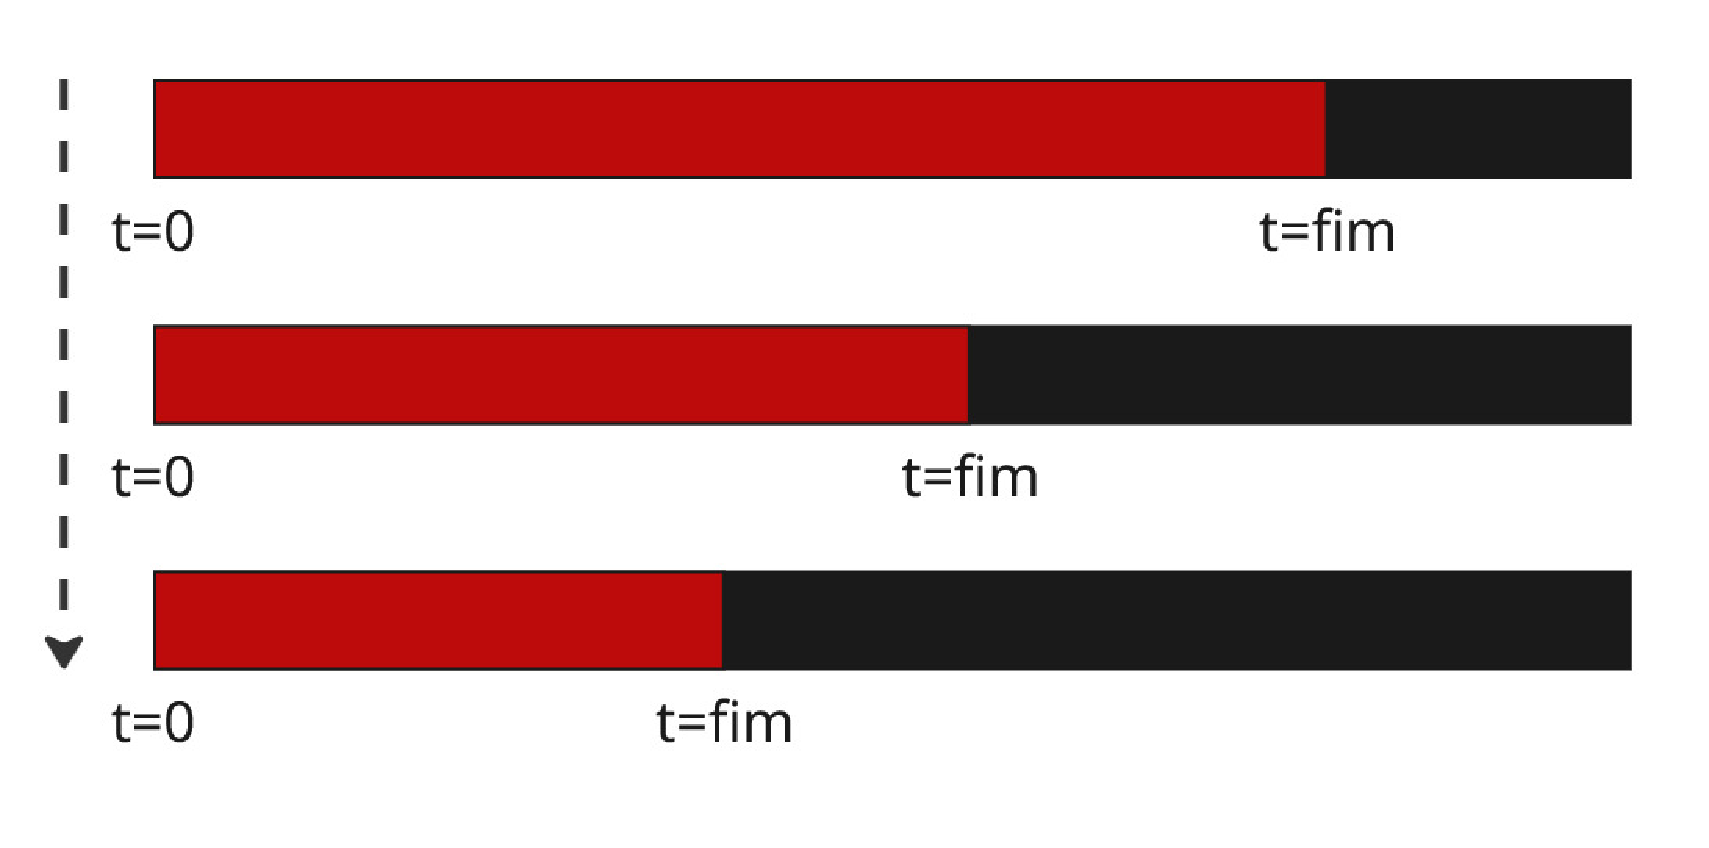
\includegraphics[width = \textwidth]{U(0_makespan)}
		\caption{Instante gerado por U(0, \textit{makespan}-duração)}
		\label{fig:U(0_makespan)}
	\end{subfigure}
	\begin{subfigure}{0.49\textwidth}
	\centering
		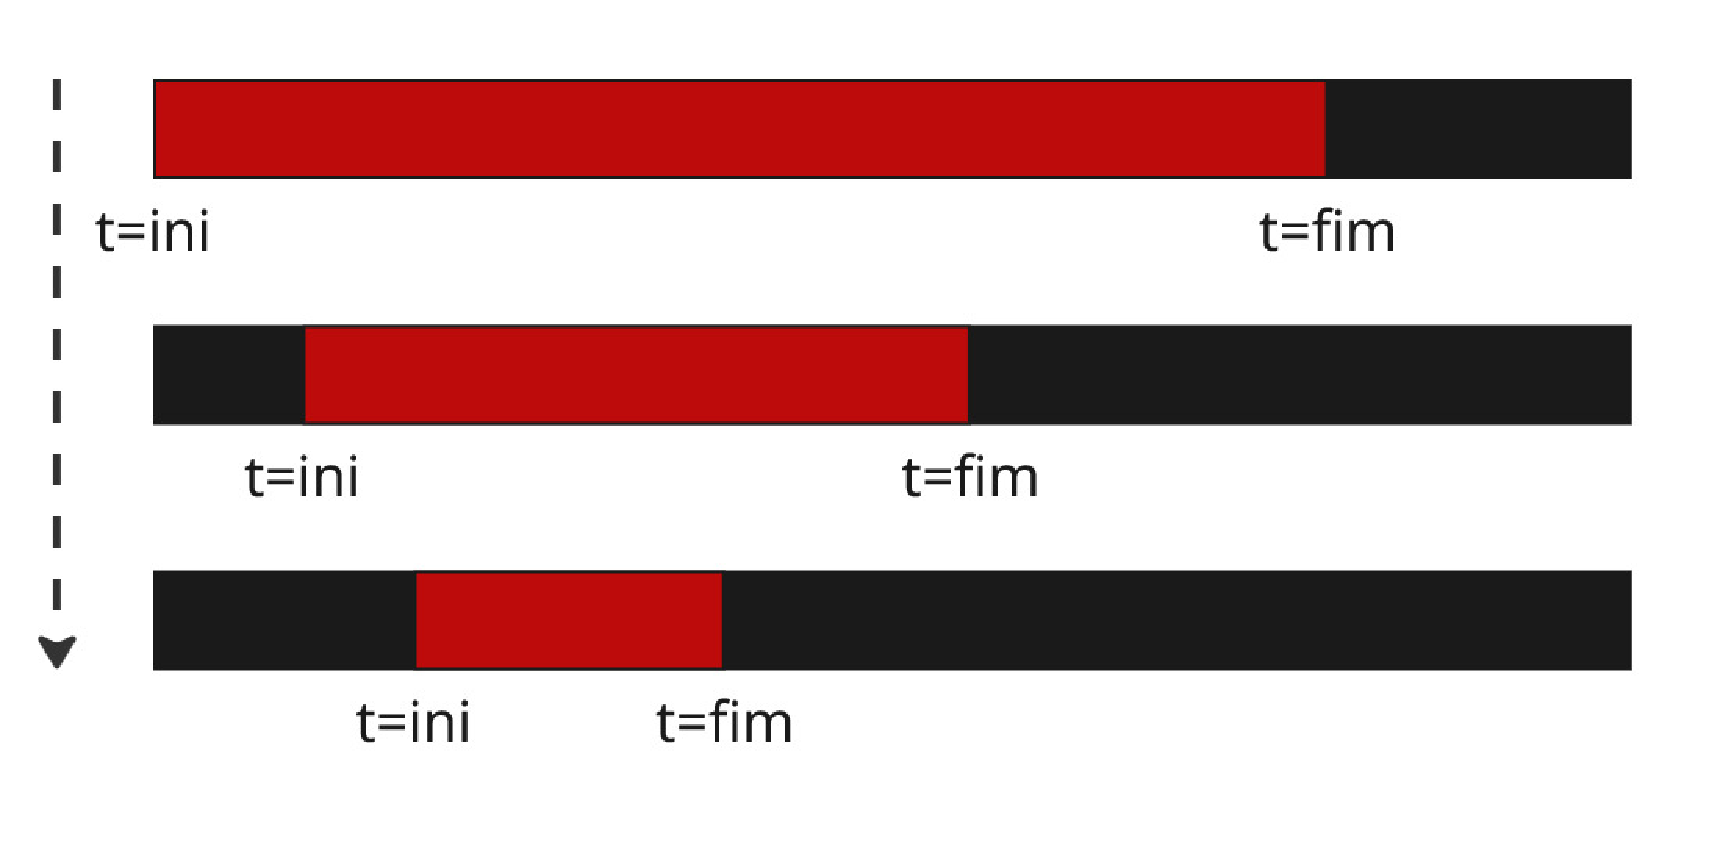
\includegraphics[width = \textwidth]{U(start_end)}
		\caption{Instante gerado por U(\textit{ini}, \textit{fim}-duração)}
		\label{fig:U(start_end)}
	\end{subfigure}
	\caption{Impacto das duas forma de gerar $t$ sobre a procura da vizinhança.}
	\label{fig:dif_uniform}
\end{figure}

O processo de modificar a solução atual $s$ de forma a obter uma nova solução $s'$ da vizinhança é resumido à figura~\ref{fig:P1M1_NGV_viz}. Sendo depois necessário atualizar a utilização dos recursos em cada instante, $u(t,p)$, recalcular $f(s')$, decidir se a nova solução é aceite ou não, atualizar a melhor solução já encontrada se for o caso, e o processo de retrocedimento. O Algoritmo~\ref{algo:P1M1_main_algo}, que se encontra no anexo~\ref{chp:algo}, descreve este processo.\\
\begin{figure}[H]
	\centering
	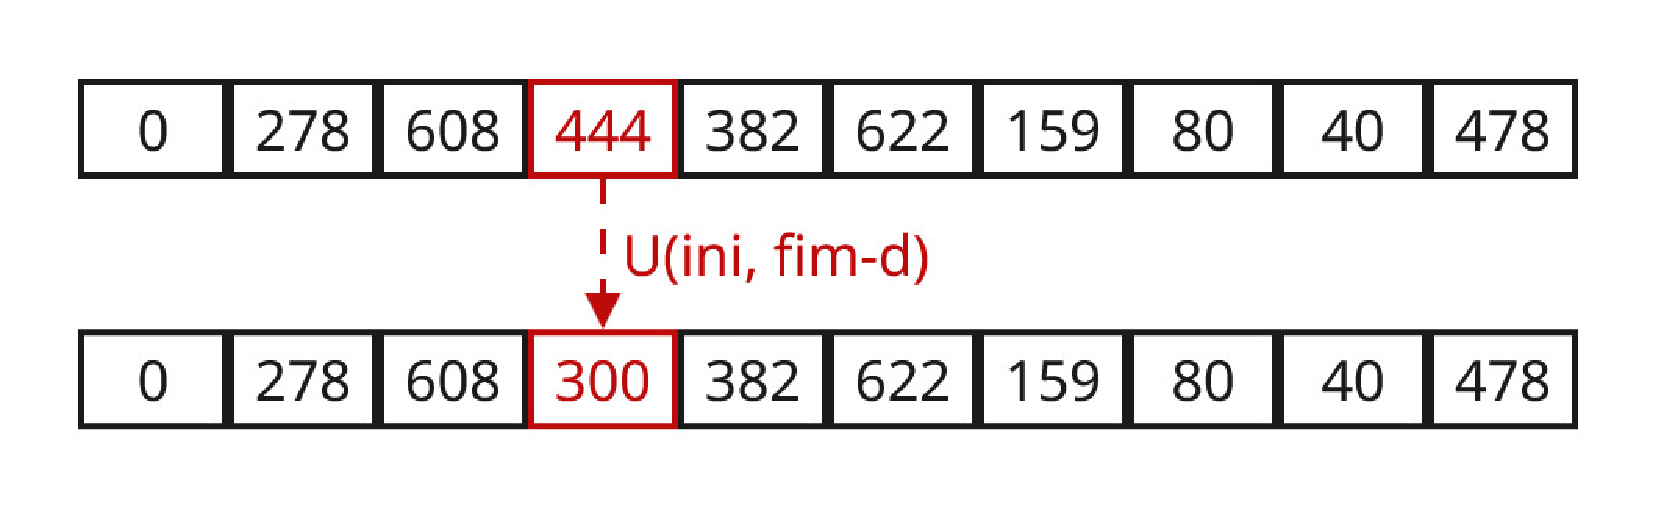
\includegraphics[width=0.5\textwidth]{P1M1_NGV_viz}
	\caption{Processo de transição da solução $s$ para a solução $s'$ para o Modelo 1.}
	\label{fig:P1M1_NGV_viz}
\end{figure}

A temperatura inicial segue o esquema \textbf{IT6}~\cite{franzinRevisitingSimulatedAnnealing2019}. Mais especificamente, gerou-se uma boa solução inicial utilizando a heurística NEH, e de seguida procedeu-se a uma caminhada aleatório da vizinhança desta solução utilizando $c=\infty$ e $L_{k}=100000$, de forma a aceitar todas as novas soluções encontradas. Definindo-se então que a temperatura inicial $c_{0}$ é dada por:
$$c_{0}=|\Delta_{avg}/log(p_{0})|$$

Onde $\Delta_{avg}$ é a diferença média entre a solução atual $s$ e o vizinho $s'$, e $p_{0}$ é a probabilidade inicial de aceitar cada solução, este último valor será uma das variáveis a estudar.\\
O critério de paragem, $CP$, utilizado foi uma modificação de \textbf{SC9}~\cite{franzinRevisitingSimulatedAnnealing2019}, onde se termina o algoritmo quando um número fixo de reduções de temperatura não geram novas soluções melhores, este valor será uma das variáveis a estudar.\\
O critério de aceitação utilizado foi o tradicional descrito por Metropolis~\cite{metropolisEquationStateCalculations1953}, ou seja, \textbf{AC1}~\cite{franzinRevisitingSimulatedAnnealing2019}.\\
O esquema de arrefecimento utilizado foi \textbf{CS2}~\cite{franzinRevisitingSimulatedAnnealing2019}, dado por $c_{k+1}=\alpha c_{k}$, $\alpha$ tipicamente é um valor perto de 1, de forma a que a redução da temperatura se dê lentamente, este valor será uma das variáveis a estudar.\\
O comprimento da temperatura, ou seja, $L_{k}$, será uma variável a estudar, adotou-se o critério \textbf{TL1}~\cite{franzinRevisitingSimulatedAnnealing2019}, considerando um número fixo de iterações durante cada redução de temperatura.\\

Existem três diferentes algoritmos considerados para a geração da solução inicial: um algoritmo \textit{greedy}; um algoritmo aleatório; e a heurística NEH. O primeiro agenda cada trabalho aleatoriamente de forma a que o fim do trabalho $i$ corresponde ao início do trabalho $i+1$, garantindo que esta solução não apresenta sobre-utilização de recursos. O segundo agenda cada trabalho de forma aleatória, sem atender à possível sobre-utilização de recursos. Verificou-se que o segundo algoritmo apresenta, na sua generalidade, melhores soluções em relação ao primeiro algoritmo.\\

Podemos observar a Figura~\ref{fig:P1M1_NGV_dif_sol_ini} de acordo com o comportamento de cada solução e o porquê de se rejeitar a heurística NEH como solução inicial. Nas Figuras~\ref{fig:P1M1_NGV_makespan_greedy},~\ref{fig:P1M1_NGV_makespan_random},~\ref{fig:P1M1_NGV_makespan_NEH} observa-se um pico da função objetivo devido à elevada temperatura inicial, que por sua vez causa a aceitação da maioria das soluções candidatas, algo necessário para haver alguma independência entre a solução inicial e a final. Com o decair da temperatura a aceitação contrai, havendo aqui grande parte da melhoria observada. Quando a temperatura é muito reduzida, \textit{SA} transforma-se numa simples procura local, ao tornar-se quase impossível aceitar soluções piores que a atual.\\

Nas Figuras~\ref{fig:P1M1_NGV_makespan_greedy_clip},~\ref{fig:P1M1_NGV_makespan_random_clip},~\ref{fig:P1M1_NGV_makespan_NEH_clip} observa-se este comportamente quando a função objetivo esta limitada a 600. As Figuras~\ref{fig:P1M1_NGV_makespan_greedy_clip},~\ref{fig:P1M1_NGV_makespan_random_clip} apresentam comportamento semelhante, contudo a Figura~\ref{fig:P1M1_NGV_makespan_NEH_clip} apresenta uma primeira solução muito boa, este facto torna-se prejudicial no decorrer do \textit{SA}, porque dificilmente haverá uma solução melhor que a inicial nas primeiras reduções de temperatura, podendo nunca melhorar até que o critério de paragem seja acionado, o que limita a qualidade das soluções encontradas.\\

As temperaturas iniciais geradas são muito elevadas, $\Delta_{avg}$ é elevado devido à grande probabilidade que cada solução gerada ter vários instantes com sobre-utilização de recursos, e devido ao elevado valor de $P$ utilizado.\\
\begin{figure}[H]
    \centering
    % Row 1
    \begin{subfigure}{0.49\textwidth}
        \centering
        \includegraphics[width=\textwidth]{P1M1_NGV_makespan_greedy}
        \caption{Função objetivo por iteração do algoritmo \textit{greedy}}
        \label{fig:P1M1_NGV_makespan_greedy}
    \end{subfigure}
    \hfill
    \begin{subfigure}{0.49\textwidth}
        \centering
        \includegraphics[width=\textwidth]{P1M1_NGV_makespan_greedy_clip}
        \caption{Função objetivo por iteração do algoritmo \textit{greedy} limitado pelo valor máximo de 600}
        \label{fig:P1M1_NGV_makespan_greedy_clip}
    \end{subfigure}
    
    % Row 2
    \begin{subfigure}{0.49\textwidth}
        \centering
        \includegraphics[width=\textwidth]{P1M1_NGV_makespan_random}
        \caption{Função objetivo por iteração do algoritmo aleatório}
        \label{fig:P1M1_NGV_makespan_random}
    \end{subfigure}
    \hfill
    \begin{subfigure}{0.49\textwidth}
        \centering
        \includegraphics[width=\textwidth]{P1M1_NGV_makespan_random_clip}
        \caption{Função objetivo por iteração do algoritmo aleatório limitado pelo valor máximo de 600}
        \label{fig:P1M1_NGV_makespan_random_clip}
    \end{subfigure}
    
    % Row 3
    \begin{subfigure}{0.49\textwidth}
        \centering
        \includegraphics[width=\textwidth]{P1M1_NGV_makespan_NEH}
        \caption{Função objetivo por iteração da heurística NEH}
        \label{fig:P1M1_NGV_makespan_NEH}
    \end{subfigure}
    \hfill
    \begin{subfigure}{0.49\textwidth}
        \centering
        \includegraphics[width=\textwidth]{P1M1_NGV_makespan_NEH_clip}
        \caption{Função objetivo por iteração da heurística NEH limitado pelo valor máximo de 600}
        \label{fig:P1M1_NGV_makespan_NEH_clip}
    \end{subfigure}
    \caption{Evolução do valor da função objetivo ao longo da otimização do problema de \textit{makespan} com o Modelo 1 ($L_{k}=5000$, $CP=100$, $\alpha=0.8$, $P=1000$, $p_{0}=0.9$).}
    \label{fig:P1M1_NGV_dif_sol_ini}
\end{figure}

Utilizar-se-à o algoritmos aleatório para gerar a solução inicial deste modelo.\\

Será de realçar ainda duas peculiaridades deste modelo. Depois da redução da temperatura, o primeiro vizinho terá de ter o seu instante $t$ gerado utilizando U(0,$T_{\max}$-duração), sendo $T_{\max}$ o somatório das durações de todos os trabalhos, caso contrário o algoritmo parece não funcionar, isto será algo a estudar no futuro.\\
Na rejeição de uma solução dever-se-ia recalcular o início e o fim da agenda, de forma a que, na próxima iteração, o novo instante gerado seja gerado com os valores de \textit{ini} e \textit{fim} relativos à solução atual. Contudo isto resulta em piores soluções finais. A Figura~\ref{fig:P1M1_NGV_walkback} pretende realçar esta diferença.\\
\begin{figure}[H]
	\centering
	\begin{subfigure}{0.49\textwidth}
	\centering
		\includegraphics[width = \textwidth]{P1M1_NGV_walkback_orig}
		\caption{Sem recálculo de textit{ini} e \textit{fim}}
		\label{fig:P1M1_NGV_walkback_orig}
	\end{subfigure}
	\begin{subfigure}{0.49\textwidth}
	\centering
		\includegraphics[width = \textwidth]{P1M1_NGV_walkback_alt}
		\caption{Com recálculo de textit{ini} e \textit{fim}}
		\label{fig:P1M1_NGV_walkback_alt}
	\end{subfigure}
	\caption{Impacto do recálculo de \textit{ini} e \textit{fim} sobre os instantes considerados na próxima iteração.}
	\label{fig:P1M1_NGV_walkback}
\end{figure}

Nas Figuras~\ref{fig:P1M1_NGV_walkback_orig},~\ref{fig:P1M1_NGV_walkback_alt} são apresentadas três agendas. A primeira é a solução atual com os possíveis instantes gerados pela distribuição uniforme a azul. A segunda apresenta a solução depois de mover o trabalho $i$ para o novo instante, admite-se que é rejeitada. A terceira apresenta uma nova solução com os possíveis instantes gerados.\\
Na Figura~\ref{fig:P1M1_NGV_walkback_orig} não se recalcula os instantes de início e de fim, desta forma os possíveis instantes gerados para a nova solução vão ser menos, o que irá dirigir a procura para a redução mais rápida de \textit{makespan}.\\
Na Figura~\ref{fig:P1M1_NGV_walkback_alt} já existe o recálculo de \textit{ini} e de \textit{fim}, ou seja, retrocedemos completamente à solução anterior.\\


\subsection{Modelo 2}

Este modelo é semelhante ao anterior, contudo existe garantia da viabilidade de cada solução durante a geração da vizinhança. Desta forma, a função objetivo é mais simples, e dada por:
$$f(s) = C_{\max}$$

Sendo $C_{\max}$ o valor de \textit{makespan} calculado como anteriormente, a diferença entre o máximo de término de cada trabalho e o valor mínimo de início de cada trabalho.\\

A codificação utilizada para este modelo é igual à do anterior. Contudo a forma de gerar a vizinhança, especificamente o novo instante $t$ que um dado trabalho deve começar, difere substancialmente. Como existe garantia da viabilidade da solução, ou seja, todas a restrições são obedecidas, não podemos selecionar qualquer instante $t$ para iniciar o trabalho $i$. Será preciso por isso um algoritmo que encontre todos os instantes onde se pode inserir o trabalho $i$ sem ocorrer sobre-utilização dos recursos. O Algoritmo~\ref{algo:P1M1_cand_gen} descreve este processo.\\

Verifica-se se para cada instante $t$ se é possível inserir o exame $i$ sem ocorrer sobre-utilização de recursos. Caso não haja, então o instante $t$ é adicionado à lista de candidatos. A partir dessa lista, é selecionado aleatoriamente um instante $t$ que será o momento no qual o trabalho $i$ começa. Foi necessário incluir na lista de candidatos um instante que se encontra-se fora da solução atual, antes do início com o valor $\max(\textit{ini}-d, 0)$ ou depois do fim, com o valor $\min(\textit{fim}+1, T_{max}-d)$. Caso contrário não se verificava nenhuma exploração de soluções, devido ao facto que os candidatos frequentemente eram apenas o mesmo instante da solução atual, causando uma temperatura inicial próxima de 0.\\

O processo de modificar a solução $s$ para uma solução $s'$ resume-se à figura~\ref{fig:P1M1_GV_viz}. Encontra-se os candidatos com o Algoritmo~\ref{algo:P1M1_cand_gen} e depois escolhe-se aleatoriamente um para o instante de começo. De seguida atualiza-se a utilização dos recursos, decide-se se a nova solução é aceite, se é a melhor já encontrada, ou se eventual é necessário retroceder. O Algoritmo~\ref{algo:P1M1_GV_main_algo} descreve este processo.\\
\begin{figure}[H]
	\centering
	\makebox[\textwidth][c]{%
		\includegraphics[width=0.5\textwidth]{P1M1_GV_viz}
	}
	\caption{Processo de transição da solução $s$ para a solução $s'$ para o Modelo 2.}
	\label{fig:P1M1_GV_viz}
\end{figure}

Foram utilizados os mesmo critérios do modelo anterior, descritos em Franzin et al.~\cite{franzinRevisitingSimulatedAnnealing2019}, ou seja, \textbf{NE1}, \textbf{UT6}, uma modificação de \textbf{SC9}, \textbf{AC1}, \textbf{CS2}, e \textbf{TL1}.\\

Foram considerados novamente as três diferentes soluções iniciais, o algoritmo \textit{greedy}, o algoritmo aleatório, e a heurística NEH.\\
A Figura~\ref{fig:P1M1_GV_dif_sol_ini} apresenta o comportamento destas três diferentes soluções iniciais sobre a função objetivo de acordo com o número de iterações. Na Figura~\ref{fig:P1M1_GV_makespan_greedy} observa-se que a primeira solução é má, mas não deve apresentar sobre-utilização de recursos devido à forma como é construida, existe depois o arrefecimento e a melhoria da solução. A Figura~\ref{fig:P1M1_GV_makespan_random} também apresenta uma solução inicial má, mas com sobre-utilização de recursos, com o decorrer do algoritmo observa-se a melhoria esperada da solução. A Figura~\ref{fig:P1M1_GV_makespan_NEH} apresenta uma boa solução inicial, que devido à temperatura inicial piora, mas como esperado existe a melhoria da solução.\\

Nas Figuras~\ref{fig:P1M1_GV_makespan_greedy_clip},~\ref{fig:P1M1_GV_makespan_random_clip} observa-se um comportamento semelhante da redução da função objetivo, com ambas a terminarem em soluções com qualidade comparável. Na Figura~\ref{fig:P1M1_GV_makespan_NEH_clip} o comportamento é semelhante, mas devido à boa solução inicial o algoritmo pode terminar prematuramente.\\

A temperatura inicial geradas neste modelo é muito inferior ao anterior, devido à inexistência de punição da sobre-utilização de recursos. A maior diferença entre duas solução vizinhas será reagendar um trabalho que se encontra inserido no meio da agenda para um dos extremos, tal que, $\Delta_{avg}$ será sempre inferior à duração do maior trabalho.\\
\begin{figure}[H]
    \centering
    % Row 1
    \begin{subfigure}{0.49\textwidth}
        \centering
        \includegraphics[width=\textwidth]{P1M1_GV_makespan_greedy}
        \caption{Função objetivo por iteração do algoritmo \textit{greedy}}
        \label{fig:P1M1_GV_makespan_greedy}
    \end{subfigure}
    \hfill
    \begin{subfigure}{0.49\textwidth}
        \centering
        \includegraphics[width=\textwidth]{P1M1_GV_makespan_greedy_clip}
        \caption{Função objetivo por iteração do algoritmo \textit{greedy} limitado pelo valor máximo de 600}
        \label{fig:P1M1_GV_makespan_greedy_clip}
    \end{subfigure}
    
    % Row 2
    \begin{subfigure}{0.49\textwidth}
        \centering
        \includegraphics[width=\textwidth]{P1M1_GV_makespan_random}
        \caption{Função objetivo por iteração do algoritmo aleatório}
        \label{fig:P1M1_GV_makespan_random}
    \end{subfigure}
    \hfill
    \begin{subfigure}{0.49\textwidth}
        \centering
        \includegraphics[width=\textwidth]{P1M1_GV_makespan_random_clip}
        \caption{Função objetivo por iteração do algoritmo aleatório limitado pelo valor máximo de 600}
        \label{fig:P1M1_GV_makespan_random_clip}
    \end{subfigure}
    
    % Row 3
    \begin{subfigure}{0.49\textwidth}
        \centering
        \includegraphics[width=\textwidth]{P1M1_GV_makespan_NEH}
        \caption{Função objetivo por iteração da heurística NEH}
        \label{fig:P1M1_GV_makespan_NEH}
    \end{subfigure}
    \hfill
    \begin{subfigure}{0.49\textwidth}
        \centering
        \includegraphics[width=\textwidth]{P1M1_GV_makespan_NEH_clip}
        \caption{Função objetivo por iteração da heurística NEH limitado pelo valor máximo de 600}
        \label{fig:P1M1_GV_makespan_NEH_clip}
    \end{subfigure}
    \caption{Evolução do valor da função objetivo ao longo da otimização do problema de \textit{makespan} com o Modelo 2 ($L_{k}=500$, $CP=100$, $\alpha=0.9$, $P=0$, $p_{0}=0.9$).}
    \label{fig:P1M1_GV_dif_sol_ini}
\end{figure}

De forma a apresentar modelos uniformes entre si, manteve-se o algoritmo aleatório na geração de soluções iniciais.\\

Este modelo tem uma peculiaridade já referida: se a lista de candidatos contiver apenas um instante entre \textit{ini} e \textit{fim}-d que não causam sobre-utilização, acabamos por verificar pouco impacto com a variação de $\alpha$ e $p_{0}$. Este facto é agravado quando, ao rejeitar uma solução, recalcula-se os valores de \textit{ini} e \textit{fim}, o que irá causar que poucos instantes além da agenda inicial sejam considerados. Ao não recalcular o início e o fim da agenda existem mais instantes disponíveis para serem selecionados. Este facto é realçado na Figura~\ref{fig:P1M1_GV_walkback}.\\
\begin{figure}[H]
	\centering
	\begin{subfigure}{0.49\textwidth}
	\centering
		\includegraphics[width = \textwidth]{P1M1_GV_walkback_orig}
		\caption{Sem recálculo de textit{ini} e \textit{fim}}
		\label{fig:P1M1_GV_walkback_orig}
	\end{subfigure}
	\begin{subfigure}{0.49\textwidth}
	\centering
		\includegraphics[width = \textwidth]{P1M1_GV_walkback_alt}
		\caption{Com recálculo de textit{ini} e \textit{fim}}
		\label{fig:P1M1_GV_walkback_alt}
	\end{subfigure}
	\caption{Impacto do recálculo de \textit{ini} e \textit{fim} sobre a lista de candidatos da próxima iteração.}
	\label{fig:P1M1_GV_walkback}
\end{figure}

Nas Figuras~\ref{fig:P1M1_GV_walkback_orig},~\ref{fig:P1M1_GV_walkback_alt} são apresentadas três agendas. A primeira é a solução atual com os dois candidatos a novo instante a azul, admite-se que o segundo candidato é escolhido. A segunda apresenta a os valores de \textit{ini} e de \textit{fim} depois de se rejeitar esta agenda. A terceira apresenta os novos candidatos.\\
Na Figura~\ref{fig:P1M1_GV_walkback_orig} não se recalcula \textit{ini} e de \textit{fim}, existe por isso um maior número de candidatos que, apesar de piorarem a solução, permitem que haja maior exploração da vizinhança. Na Figura~\ref{fig:P1M1_GV_walkback_alt} já se recalcula \textit{ini} de \textit{fim}, o que limita o número de candidatos possíveis e diminui a exploração da vizinhança que ocorre.\\

\subsection{Modelo 3}

Este modelo continua a garantir a viabilidade de cada solução considerada, por isso a função objetivo não será mais que o valor de \textit{makespan}.\\
Contudo, a codificação utilizada difere fortemente dos modelos anteriores. Em vez de representar uma solução pelo tempo de começo de cada trabalho, a solução é representada pela sequência pela qual se agenda cada trabalho, iremos representar esta sequência por $\pi$.\\
Esta sequência pouca informação fornece por si só, nomeadamente está ausente o instante em que cada trabalho deve começar. Para tal é necessário um algoritmo auxiliar que descodifica a sequência de forma a obter a agenda, a este algoritmo chamamos de \textit{timetabling}. Existem vários algoritmos utilizados para este fim, contudo apenas dois vão ser descritos com mais profundidade, \textit{left-shift timetabling} e \textit{enhanced left-shift timetabling}~\cite{dengPopulationbasedIteratedGreedy2020}.\\

O Algoritmo~\ref{algo:earliest_t} permite encontrar o instante de tempo $t$ mais cedo onde é possível agendar o trabalho $i$ que se está a agendar. A forma de como isto é feito é algo bruta, pois percorre-se cada instante $t$ e insere-se o trabalho $i$ verificando se existe, ou não, sobre-utilização de recursos, caso não haja retorna-se $t$. Este algoritmo consome a maioria do tempo computacional deste modelo.\\
Uma adaptação pode ser utilizada, caso se conheça quais os recursos limitantes, ou seja, aqueles que mais provavelmente originaram sobre-utilização, pode-se primeiro verificar apenas esses recursos, e só depois verificar os restantes. Esta adaptação foi implementada, utilizando como recursos limitantes SCG e TM, aumentando a probabilidade de rejeitar um instante no início da verificação.\\

O Algoritmo~\ref{algo:left-shift-TT} encontra, para cada elemento da solução, o instante de tempo mais cedo onde este pode ser inserido, modificando a matriz de utilização de recursos. Na literatura admite-se que assegurar que $t_{\pi[i]} \geq t_{\pi[i-1]}$, ou seja que cada elemento da sequência deve começar no mesmo instante ou depois do elemento anterior, tende a reduzir a qualidade da solução, por isso esta característica não é assegurada.\\
O Algoritmo~\ref{algo:enh-left-shift-TT} é semelhante, para cada elemento da sequência $\pi=\pi[0],\ldots, \pi[n-1]$, encontra o instante mais cedo onde cada elemento pode ser inserido. Ao mesmo tempo faz este processo para a sequência inversa, $\pi=\pi[n-1],\ldots, \pi[0]$, em que cada trabalho também é o inverso, ao inverter $\delta$. Não há a garantia que um ou outro algoritmo é melhor, mas existe a possibilidade de serem geradas soluções melhores com este passo adicional. Em contrapartida, o tempo computacional associado à descodificação da solução aproximadamente duplica.\\

Para demonstrar a diferença entre estes dois algoritmos irá utilizar-se o exemplo apresentado por Ying e Lin~\cite{yingSolvingNowaitJobshop2020}, que geraram um pequeno problema \textit{No-Wait Job-Shop}. Para cada um dos quatro trabalhos deste problema, a Tabela~\ref{tab:P1M2_GV_examp} apresenta a sequência das operações que devem ser realizadas, e o respetivo tempo de processamento. Ou seja, o trabalho $I_{1}$ primeiro passa pelo recurso 4 com tempo de processamento de 7 unidades de tempo, a segunda operação será no recurso 3 durante 9 unidades de tempo, a terceira será no recurso 1 durante 8 unidades de tempo, a quarta operação será no recurso 2 durante 4 unidades de tempo.\\

\begin{table}[H]
\caption{Problema definido pela operações de cada trabalho e os recursos necessários e tempo de processamento, apresentado por Ying e Lin~\cite{yingSolvingNowaitJobshop2020}.}
\label{tab:niveis_P1}
\centering
\begin{tabular}{c|llll}
Trabalho & \multicolumn{4}{c}{Sequência de recursos (tempo)} \\ \hline
$I_{1}$  & 4(7)$\to$ & 3(9)$\to$ & 1(8)$\to$ & 2(4)          \\
$I_{2}$  & 1(4)$\to$ & 4(8)$\to$ & 2(2)$\to$ & 3(4)          \\
$I_{3}$  & 3(5)$\to$ & 2(7)$\to$ & 1(1)$\to$ & 4(4)          \\
$I_{4}$  & 4(3)$\to$ & 2(1)$\to$ & 1(2)$\to$ & 3(3)
\end{tabular}
\label{tab:P1M2_GV_examp}
\end{table}

O exemplo dado utiliza a sequência 3-4-1-2, ou seja, agenda-se o mais cedo possível o trabalho 3, depois o trabalho 4, de forma consecutiva sem garantir que $t_{3}\leq t_{4}\leq t_{1}\leq t_{2}$. Pode ver-se, na Figura~\ref{fig:P1M2_GV_paper_example} as duas fases do Algoritmo~\ref{algo:enh-left-shift-TT}, com a agenda \textit{forward} a utilizar a sequência original, e a agenda \textit{backward} com a sequência inversa e com cada trabalho também invertido, é evidente que das duas agendas apresentadas iremos escolher aquela que possua o menor \textit{makespan}, sendo neste caso a agenda \textit{forward}.\\
\begin{figure}[H]
	\centering
	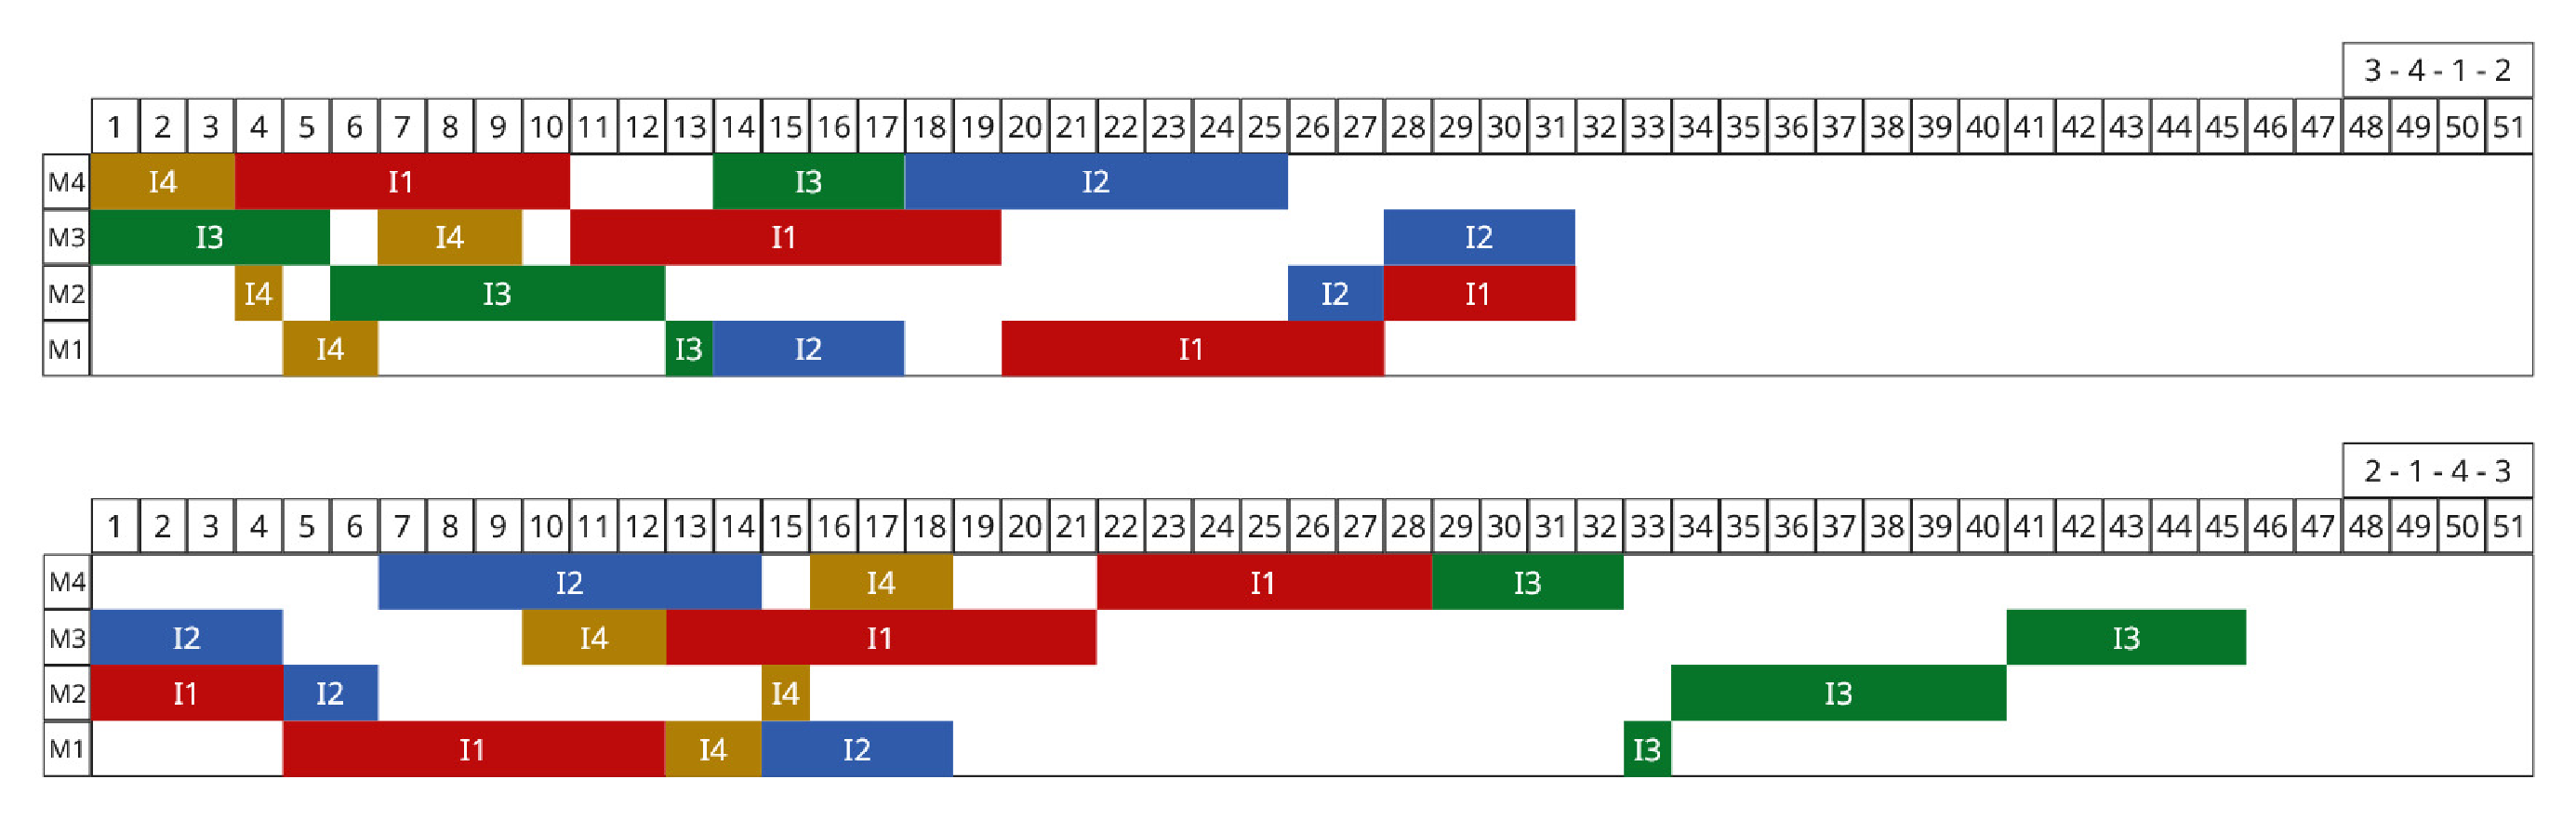
\includegraphics[width = \textwidth]{P1M2_GV_paper_example}
	\caption{Exemplo da solução 3-4-1-2}
	\label{fig:P1M2_GV_paper_example}
\end{figure}

Novamente, observa-se outro exemplo de uma solução na figura~\ref{fig:P1M2_GV_paper_better_inverse}, agora com a sequência 2-3-1-4, com a agenda \textit{forward} e a \textit{backward}, respetivamente. Este exemplo serve para demonstrar a utilidade de representar a mesma solução com mais de um algoritmo de \textit{timetabling}. Podendo transformar uma solução aparente má numa boa solução.\\
\begin{figure}[H]
	\centering
	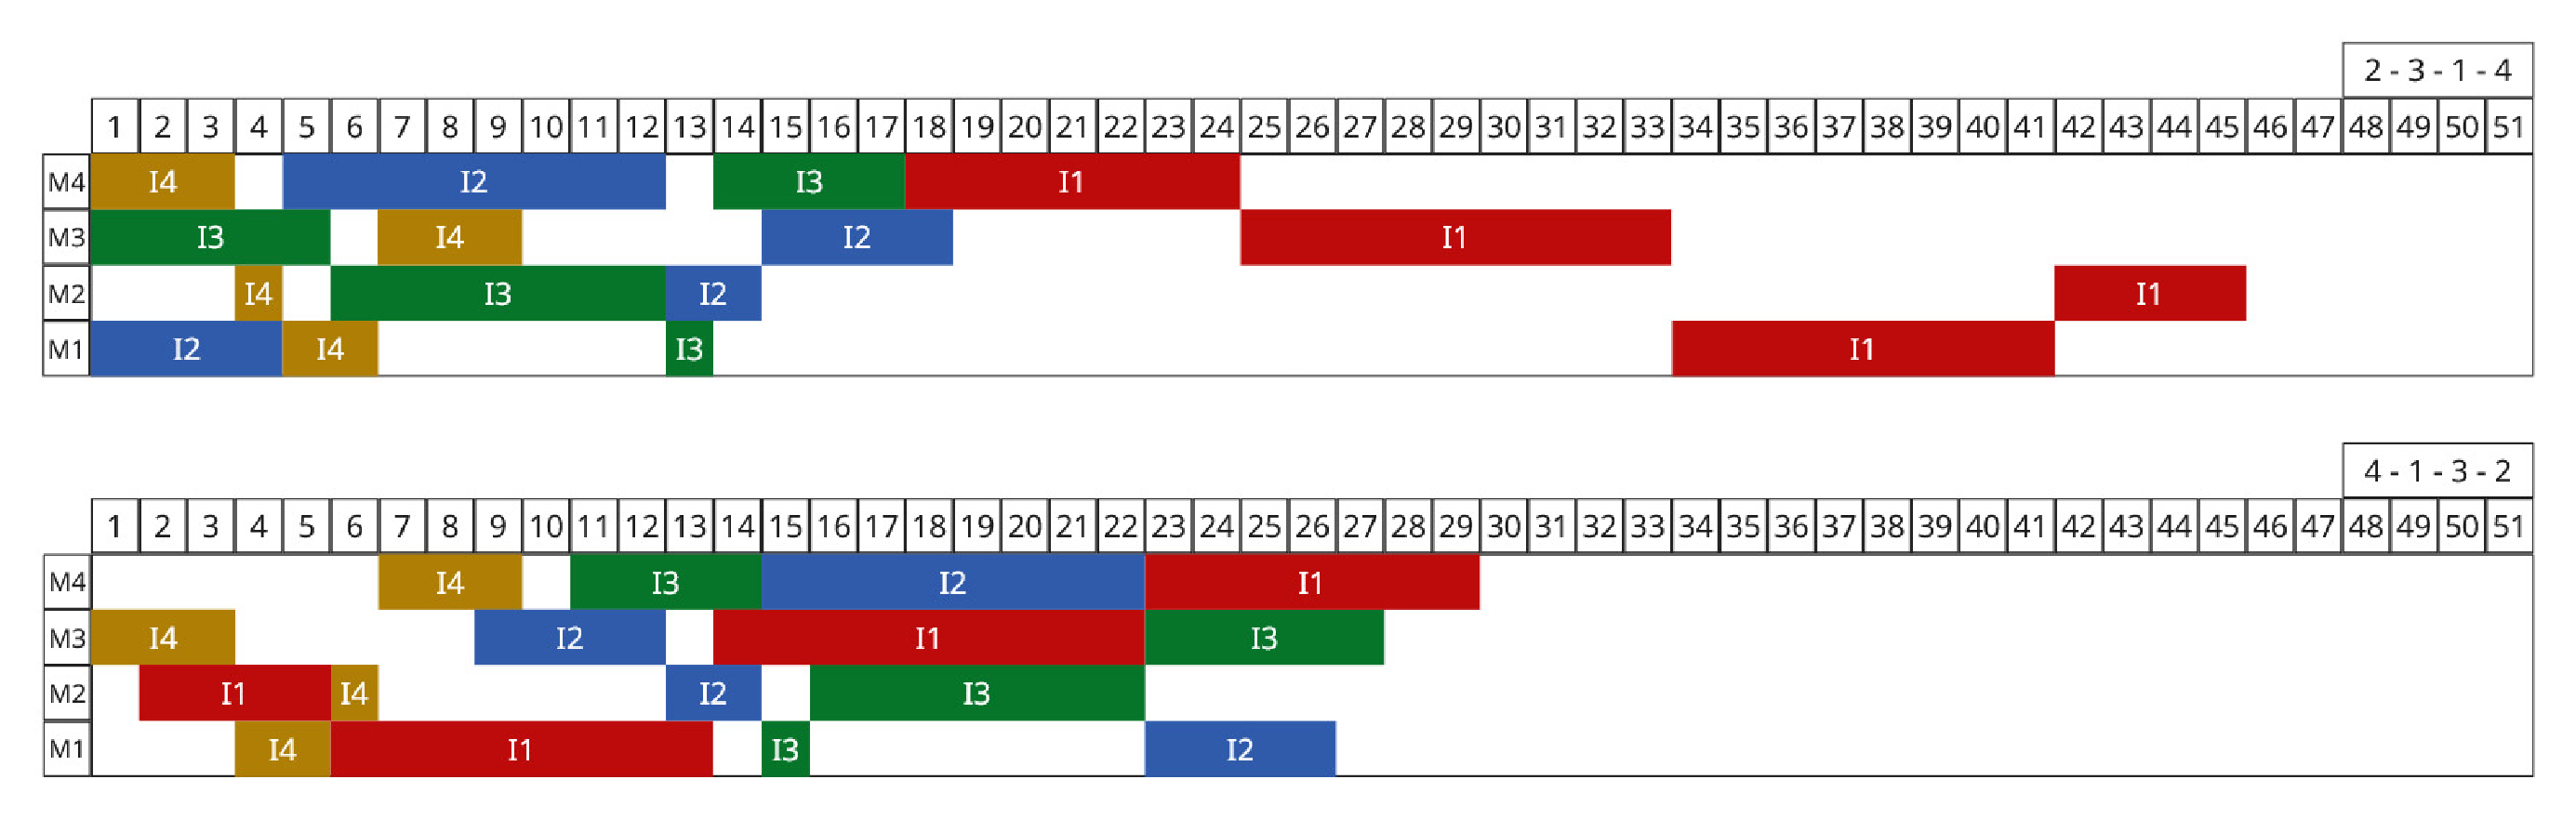
\includegraphics[width = \textwidth]{P1M2_GV_paper_better_inverse}
	\caption{Exemplo da solução 2-3-1-4}
	\label{fig:P1M2_GV_paper_better_inverse}
\end{figure}

Por sua vez, a vizinhança de uma solução pode ser gerada de três formas, com várias variantes. Através de uma troca de índice entre trabalhos, Figura~\ref{fig:P1M2_GV_swap}. Através da retirada de um trabalho e a sua inserção noutro índice da sequência, Figura~\ref{fig:P1M2_GV_insert}. Através da inversão de uma sub-sequência de trabalhos, Figura~\ref{fig:P1M2_GV_invert}. Não existe, contudo, nenhuma evidência que um dos métodos é superior ao outro, na continuação iremos utilizar a troca de trabalhos. O Algoritmo~\ref{algo:P1M2_GV_main_algo} apresenta o processo de gerar a vizinhança, de avaliação, rejeição ou aceitação, atribuição da melhor solução, e possível retrocesso.\\
\begin{figure}[H]
	\centering
	\begin{subfigure}{0.49\textwidth}
	\centering
		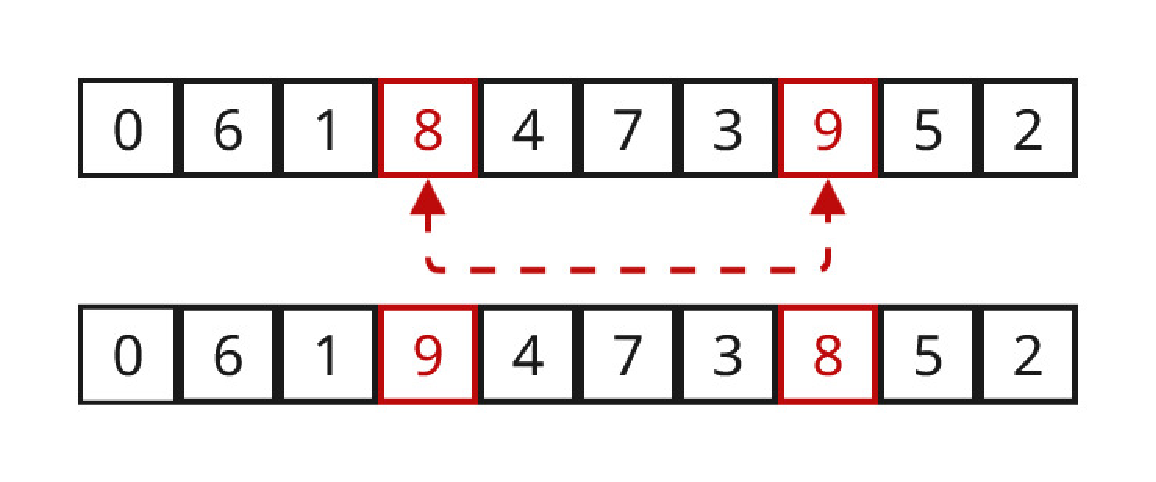
\includegraphics[width = \textwidth]{P1M2_GV_swap}
		\caption{Troca entre trabalhos.}
		\label{fig:P1M2_GV_swap}
	\end{subfigure}
	\begin{subfigure}{0.49\textwidth}
	\centering
		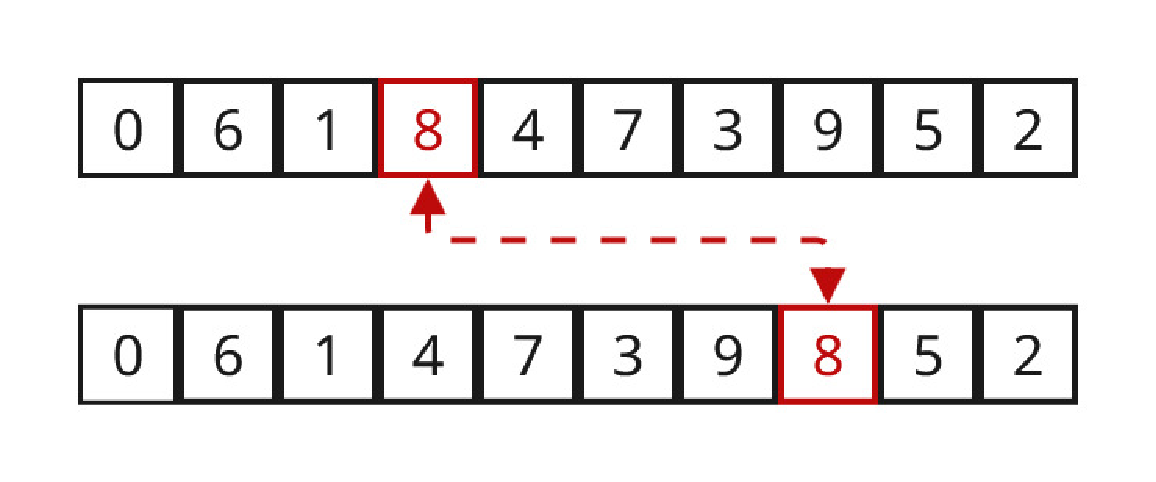
\includegraphics[width = \textwidth]{P1M2_GV_insert}
		\caption{Inserção de trabalho.}
		\label{fig:P1M2_GV_insert}
	\end{subfigure}
	\begin{subfigure}{0.49\textwidth}
	\centering
		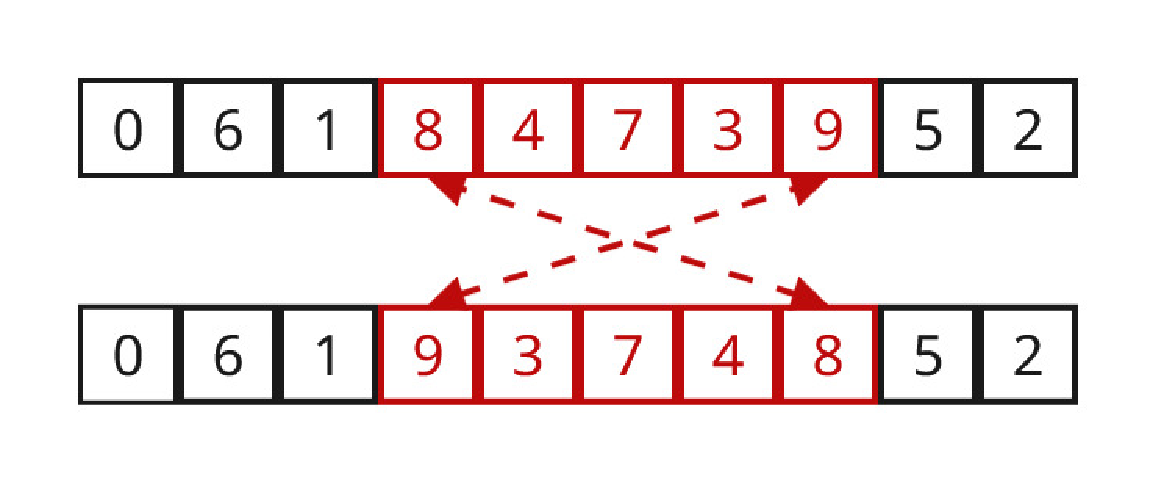
\includegraphics[width = \textwidth]{P1M2_GV_invert}
		\caption{Inversão de sub-sequência de tranalhos.}
		\label{fig:P1M2_GV_invert}
	\end{subfigure}
	\caption{Processo de transição da solução $s$ para a solução $s'$ para o Modelo 3.}
	\label{fig:P1M2_GV_gen}
\end{figure}

Como o problema aqui definido contém vários trabalhos do mesmo tipo, ou seja, existem vários exames que são iguais, é essencial verificar que ao trocar trabalhos não se comete o erro destes serem do mesmo tipo. Caso contrário está-se a desperdiçar tempo computacional com soluções que são iguais.\\

Foram utilizados os mesmo critérios do modelo anterior, descritos em Franzin et al.~\cite{franzinRevisitingSimulatedAnnealing2019}, ou seja, \textbf{NE1}, \textbf{UT6}, uma modificação de \textbf{SC9}, \textbf{AC1}, \textbf{CS2}, e \textbf{TL1}.\\

A geração da solução inicial é diferente dos modelos anterior, devido à codificação diferente. A forma mais simples de gerar uma solução será pela escolha aleatória de uma sequência, existindo sempre garantia da viabilidade da solução graças ao algoritmo de \textit{timetabling}. Também será possível utilizar a heurística de NEH para este fim.\\
A Figura~\ref{fig:P1M2_GV_dif_sol_ini} apresenta o comportamento destas duas formas de gerar a solução inicial relativamente à função objetivo com o decorrer das iteração. Nas Figuras~\ref{fig:P1M2_GV_makespan_random},~\ref{fig:P1M2_GV_makespan_NEH} observa-se um comportamento semelhante entre si, contudo este difere do observado nos modelos anteriores. Continua-se a verificar a tendência de obter soluções más no início do algoritmo que tendem a melhorar com o arrefecimento, contudo observa-se maior variação entre iterações sequenciais.\\

O informação retirada das Figuras~\ref{fig:P1M2_GV_makespan_random_clip},~\ref{fig:P1M2_GV_makespan_NEH_clip} é menos relevante do que nos problemas anteriores devido à menor amplitude na qualidade das soluções observadas.\\

A temperatura inicial gerada neste modelo é superior à do Modelo 2 mas ainda muito inferior à do Modelo 1. Este facto deve-se ao grande impacto sobre o \textit{makespan} que um trabalho pode ter ao ser colocado no lugar errado da sequência.\\
\begin{figure}[H]
    \centering    
    % Row 1
    \begin{subfigure}{0.49\textwidth}
        \centering
        \includegraphics[width=\textwidth]{P1M2_GV_makespan_random}
        \caption{Função objetivo por iteração do algoritmo aleatório}
        \label{fig:P1M2_GV_makespan_random}
    \end{subfigure}
    \hfill
    \begin{subfigure}{0.49\textwidth}
        \centering
        \includegraphics[width=\textwidth]{P1M2_GV_makespan_random_clip}
        \caption{Função objetivo por iteração do algoritmo aleatório limitado pelo valor máximo de 600}
        \label{fig:P1M2_GV_makespan_random_clip}
    \end{subfigure}
    
    % Row 2
    \begin{subfigure}{0.49\textwidth}
        \centering
        \includegraphics[width=\textwidth]{P1M2_GV_makespan_NEH}
        \caption{Função objetivo por iteração da heurística NEH}
        \label{fig:P1M2_GV_makespan_NEH}
    \end{subfigure}
    \hfill
    \begin{subfigure}{0.49\textwidth}
        \centering
        \includegraphics[width=\textwidth]{P1M2_GV_makespan_NEH_clip}
        \caption{Função objetivo por iteração da heurística NEH limitado pelo valor máximo de 600}
        \label{fig:P1M2_GV_makespan_NEH_clip}
    \end{subfigure}
    \caption{Evolução do valor da função objetivo ao longo da otimização do problema de \textit{makespan} com o Modelo 3 ($L_{k}=500$, $CP=100$, $\alpha=0.9$, $P=0$, $p_{0}=0.9$, \textit{left-shift timetabling}, geração de vizinhos através de troca).}
    \label{fig:P1M2_GV_dif_sol_ini}
\end{figure}

Este modelo acaba por ser dividido em dois problemas distintos, o problema de sequenciamento e o de \textit{timetabling} já discutido. Sem um bom algoritmo de \textit{timetabling} a melhor solução possível não será a ótima, mas a sequência é o que realmente define a solução.\\










\section{Problema do número de trabalhos}

Este problema é definido por apresentar um período, ou \textit{makespan}, fixo, com capacidades máximas de recursos pré-definidas, mas com a quantidade de trabalhos a maximizar. Esta otimização poderá ser uma soma dos trabalhos que se inserem no período pré-definido ou utilizar-se um peso para cada trabalho de forma a representar as escolhas do decisor. Este pode pode ser definido antes de começar o algoritmo ou ser um valor que se adapta ao longo deste.\\
Por exemplo, se existir a possibilidade de agendar 20 trabalhos do tipo $A$, ou em contrapartida agendar 19 trabalhos do tipo $A$ e 1 do tipo $B$, pode ser benéfico assegurar que a segunda opção seja valorizada sobre a primeira. Semelhantemente, o somatório sem consideração de pesos, beneficia a escolha de exames de curta duração sobre exames de longa duração.\\

A próxima formulação é derivada da $MILP-\delta$ apresentada na secção anterior:\\

Conjuntos:\\
O conjunto de trabalhos $I, i \in I := (1, \ldots, n)$ \\
O conjunto de recursos-tipo $R, p \in R := (1, \ldots, R_{\max})$ \\
O conjunto de instantes de tempo $T, t \in T := (1, \ldots, T_{\max})$ \\

Parâmetros:\\
$\rho_{i}$ é duração do trabalho $i$ \\
$\delta_{i}(u,p)$ é a quantidade de recursos do tipo $p$ necessários a um offset de $u$ instantes de tempo no trabalho $i$\\
$C_{p}$ é a capacidade do recurso $p$ \\

Variáveis de Decisão: \\
$Y_{i}$ é uma variável binária com valor 1 se o trabalho $i$ estiver agendado, caso contrário tem valor 0 \\
$Z_{t,i}$ é uma variável binária com valor 1 se o trabalho $i$ começar no instante $t$, caso contrário tem valor 0 \\

Função Objetivo:
\begin{align}
\min \sum -Y \label{eq:15}
\end{align}

Sujeito a:
\begin{align}
&\sum^{T_{\max}-\rho_{i}+1}_{t=0}Z_{t,i} = Y \quad \forall i \label{eq:16} \\
&\sum_{i}\sum^{\min(t, T_{\max}-\rho_{i})}_{\tau=\max(0, t-\rho_{i}+1)}\delta_{i}(t-\tau,p)Z_{\tau,i} \leq C_{p} \quad \forall t,p \label{eq:17}
\end{align}
A função objetivo (~\ref{eq:15}) minimiza o \textit{makespan} dos trabalho.\\
A restrição (~\ref{eq:16}) garante que só existe um instante de começo do trabalho $i$ quando este exame estiver agendado, caso contrário não existe instante de começo.\\
A restrição (~\ref{eq:17}) garante que não há sobre utilização de recursos, ao verificar para cada instante $t$ quais trabalhos estão a ser executados e em que fase este se encontra, garantindo que em cada instante não há sobre-utilização de recursos.\\

O problema é de minimização de forma a manter a coerência entres os valores obtidos com esta formulação e os valores obtidos em \textit{SA}. Para a função objetivo considerou-se apenas o somatório dos exames sem nenhum peso adicional. Assegura-se que todos os exames agendados se encontram dentro do período através da definição de $T_{\max}$.\\

De seguida foram desenvolvidos três modelos análogos ao problema anterior, dois deles com a codificação dos instantes de começo de cada trabalho, e o terceiro modelo com a solução representada pela sequência de escalonamento.\\

\subsection{Modelo 1}

Para começar, será necessário definir a vizinhança. Ao contrário do problema anterior, onde todos os trabalhos estavam agendados e apenas era necessário definir o instante de começo de cada um. Este problema requer definir quais exames são agendados e em que instante devem começar, para tal existem três movimentos diferentes que podem ocorrer.\\
O mais comum será a definição de um novo instante de começo $t$ para um dado trabalho $i$ já pertencente à agenda, sem assegurar a viabilidade da solução.\\
Por outro lado, tem de existir alguma probabilidade de remover algum exame $i$ pertencente à agenda, como também adicionar um novo exame, esta adição considera-se que ocorre sem garantia de viabilidade.\\
A função objetivo que pretendemos minimizar é dada por:
$$f(s) = \sum -Y + P \sum_{t=0}^{T_{\max}-1}\sum_{p}v(t,p)$$

Onde $Y$ é uma variável binária com os trabalhos agendados, $P$ é a punição relativamente à sobre-utilização de recursos, e com $v(t,p)$ a representar se existe ou não sobre-utilização do recurso $p$ no instante $t$.\\

Para a definição do novo vizinho são necessários três componente: $m,i,t$. Tal que $m$ represente que movimento se realiza, $i$ o trabalho a alterar, e $t$ o instante. Considera-se que o movimento 0 seja da mudança do instante de começo $t$ para um trabalho $i$. O movimento 1 implica a remoção do trabalho $i$ da agenda. O movimento 2 adiciona-se o trabalho $i$ à agenda no instante de começo $t$.\\
Para o movimento 0, deve-se ter o cuidado de apenas selecionar um trabalho que já se encontre na agenda atual, por sua vez o instante $t$ pode ser gerado por U(0, $T_{\max}$-duração), não existindo necessidade de utilizar U(\textit{ini}, \textit{fim}-d). Para o movimento 1, também é necessário ter o cuidado de apenas selecionar um trabalho $i$ que se encontre na agenda. Para o movimento 2, o trabalho $i$ a adicionar não deve pertencer à agenda, e o instante de começo $t$ é gerado por U(0, $T_{\max}$-d). Esta dinâmica pode ser representada pela figura~\ref{fig:P2M1_NNGV_gen}. O Algoritmo~\ref{algo:P2M1_main_algo} apresenta como se deve proceder na escolha do movimento e que passos são necessários para gerar a vizinhança, avaliá-la, aceitá-la ou rejeitá-la. O Algoritmo~\ref{algo:P2M1_main_algo_rollback} apresenta como se deve fazer o retrocesso de cada movimento caso se rejeite a solução.\\
\begin{figure}[H]
	\centering
	\begin{subfigure}{0.49\textwidth}
	\centering
		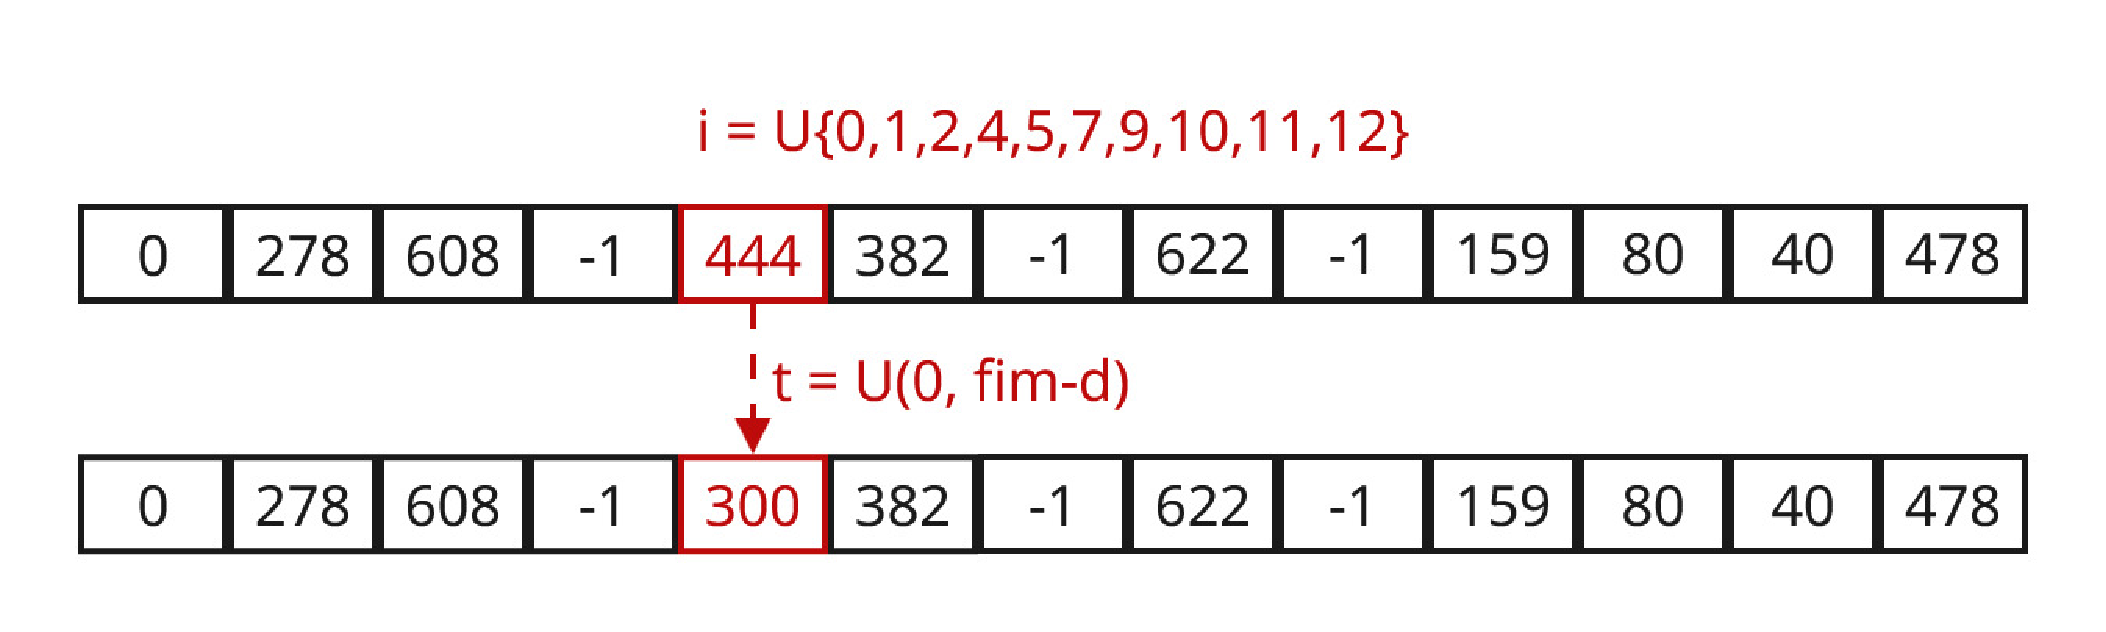
\includegraphics[width = \textwidth]{P2M1_NNGV_M0}
		\caption{Movimento 0}
		\label{fig:P2M1_NNGV_M0}
	\end{subfigure}
	\begin{subfigure}{0.49\textwidth}
	\centering
		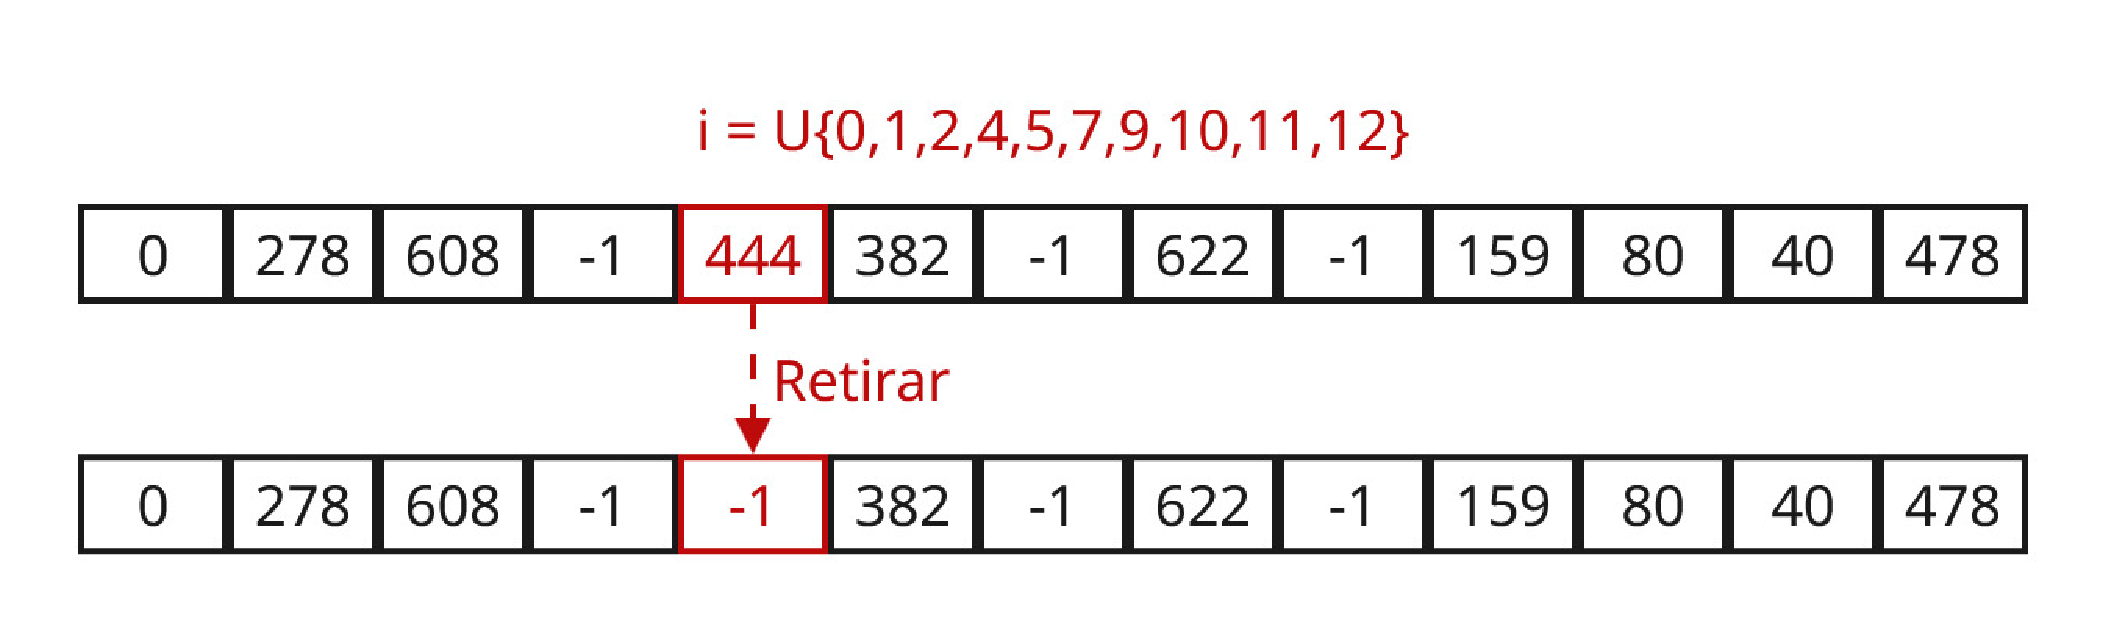
\includegraphics[width = \textwidth]{P2M1_NNGV_M1}
		\caption{Movimento 1}
		\label{fig:P2M1_NNGV_M1}
	\end{subfigure}
	\begin{subfigure}{0.49\textwidth}
	\centering
		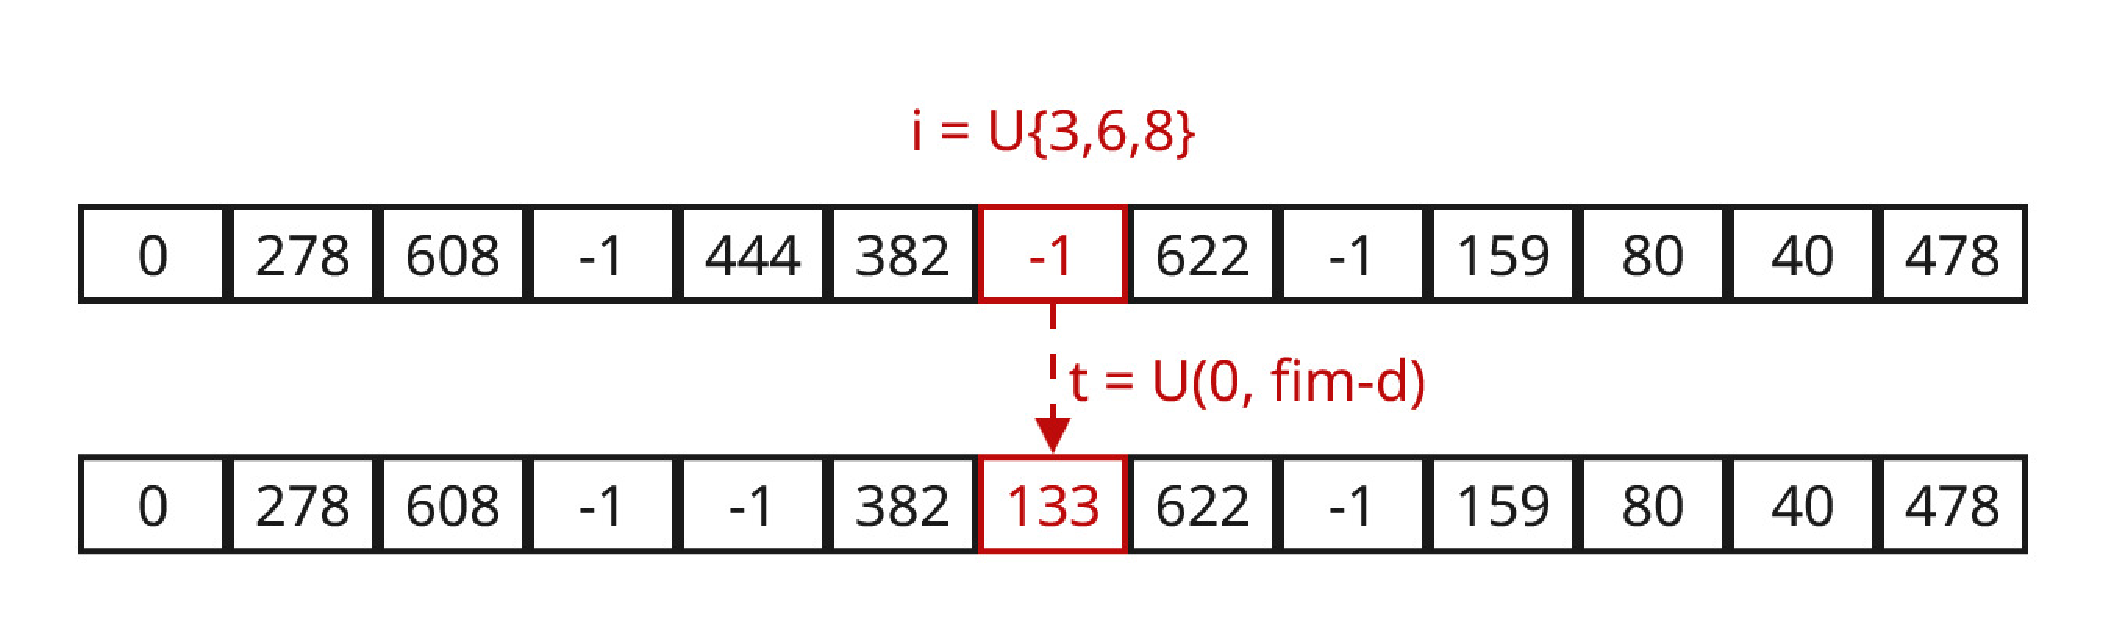
\includegraphics[width = \textwidth]{P2M1_NNGV_M2}
		\caption{Movimento 2}
		\label{fig:P2M1_NNGV_M2}
	\end{subfigure}
	\caption{Processo de transição da solução $s$ para a solução $s'$ para o Modelo 1.}
	\label{fig:P2M1_NNGV_gen}
\end{figure}

Cada um destes movimentos ocorrem de forma aleatória com uma probabilidade pré-definida. De forma a diminuir o número de variáveis a testar, consideramos que a probabilidade de ocorrer o movimento 1 e o movimento 2 é de 5\% cada.\\

Relativamente à temperatura inicial, gerou-se uma boa solução através da heurística NEH, de forma a tentar agendar todos os trabalhos dentre do tempo limite de $T_{\max}$, aqueles que de facto terminam antes de $T_{\max}$ são contabilizados. Procedesse a uma caminhada aleatória com $c=\infty$ e $L_{k}=100000$ para que se aceite todos as soluções visitadas. Finalmente a temperatura inicial é dada por $c_{0}=|\Delta_{avg}/log(p_{0})|$.\\

Para a solução inicial consideraram-se dois algoritmos aleatórios. A Figura~\ref{fig:P2M1_NNGV_dif_sol_ini} apresenta a função objetivo ao longo do número de iteração para cada uma das soluções iniciais.\\

A solução inicial que origina a Figura~\ref{fig:P2M1_NNGV_n_exams_random} agenda todos os trabalhos de forma aleatória, enquanto a solução inicial que origina a Figura~\ref{fig:P2M1_NNGV_n_exams_random_alt} agenda um número aleatório de trabalhos. Em ambos os casos observa-se um comportamento semelhante ao já descrito. Ocorre o aumento inicial da função objetivo, mesmo que mais acentuado na Figura~\ref{fig:P2M1_NNGV_n_exams_random}, seguido do declínio com o arrefecimento da temperatura.\\

As Figuras~\ref{fig:P2M1_NNGV_n_exams_random_clip},~\ref{fig:P2M1_NNGV_n_exams_random_alt_clip} não diferem desta análise. Ocorre um rápido declínio da função objetivo com o arrefecimento da temperatura até que se congela e $CP$ seja ativado, dando o algoritmo como terminado.\\

Analogamente ao Modelo 1 do problema de \textit{makespan}, a temperatura inicial é bastante alto. Contudo é menor devido às menores diferenças entre soluções vizinhas e ao menor valor de $P$ utilizado. Apesar do algoritmo aleatório alternativo apresentar melhor solução, na combinação de níveis descrita pela Figura~\ref{fig:P2M1_NNGV_dif_sol_ini}, de forma a manter a uniformidade utilizar-se-à o algoritmo aleatório para gerar as soluções iniciais.\\
\begin{figure}[H]
    \centering
    % Row 1
    \begin{subfigure}{0.49\textwidth}
        \centering
        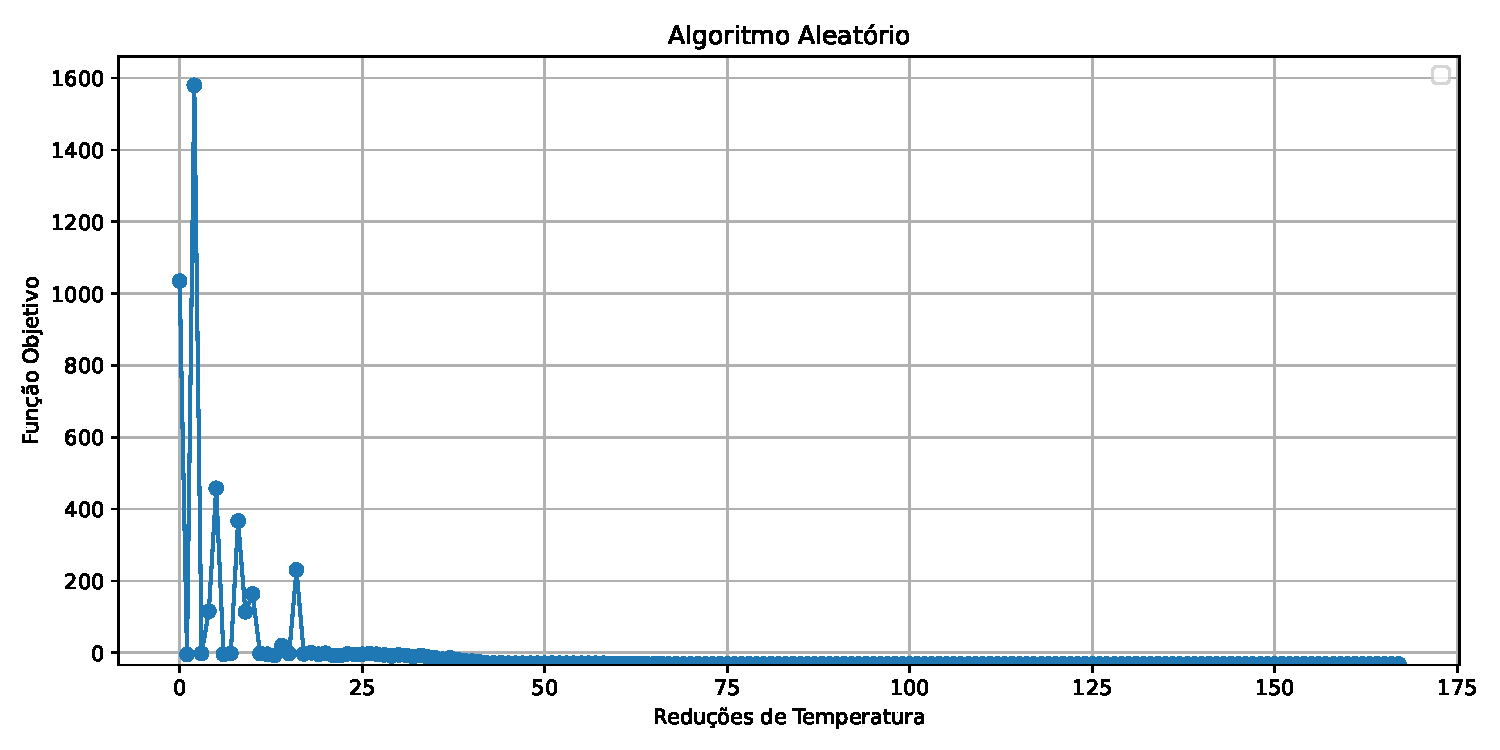
\includegraphics[width=\textwidth]{P2M1_NNGV_n_exams_random}
        \caption{Função objetivo por iteração do algoritmo aleatório}
        \label{fig:P2M1_NNGV_n_exams_random}
    \end{subfigure}
    \hfill
    \begin{subfigure}{0.49\textwidth}
        \centering
        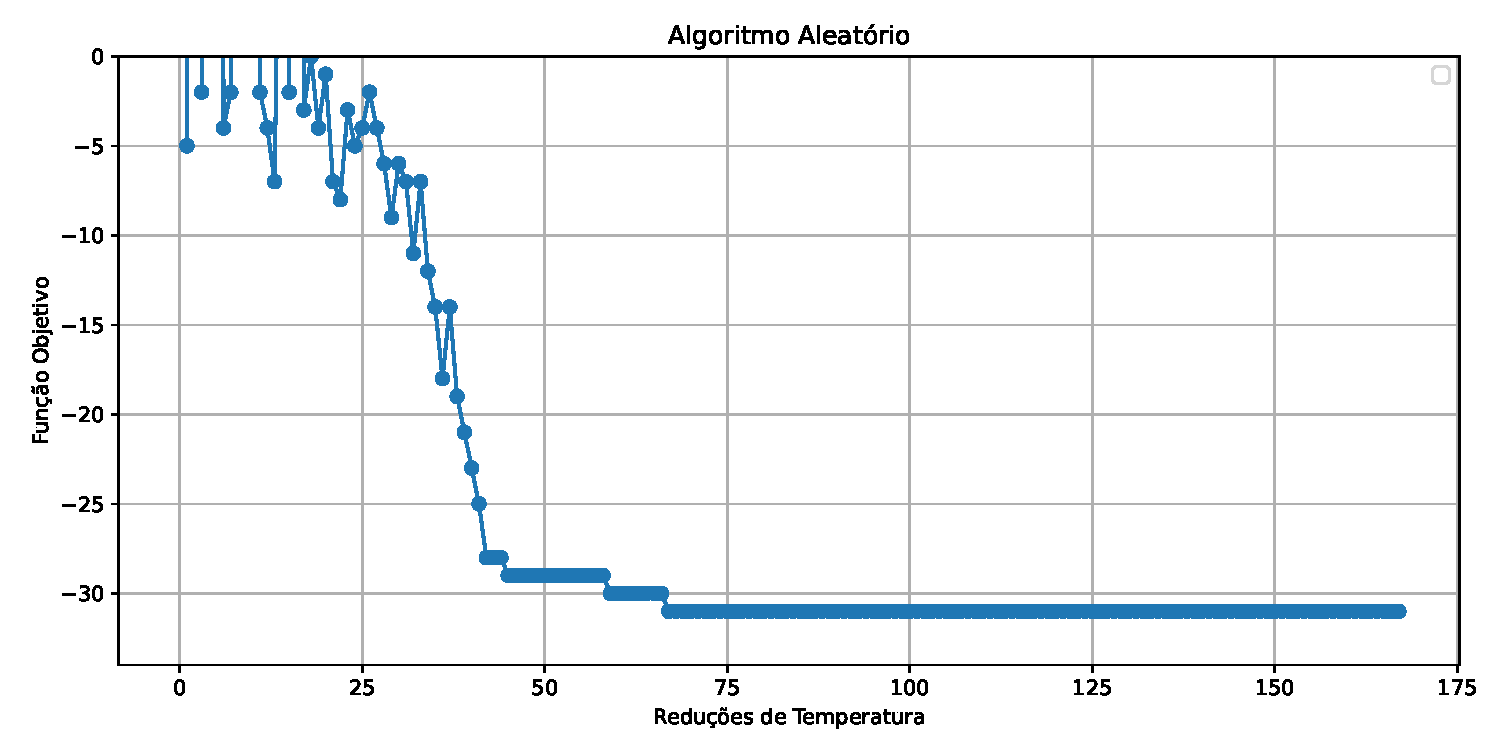
\includegraphics[width=\textwidth]{P2M1_NNGV_n_exams_random_clip}
        \caption{Função objetivo por iteração do algoritmo aleatório limitado pelo valor máximo de 0}
        \label{fig:P2M1_NNGV_n_exams_random_clip}
    \end{subfigure}
    
    % Row 2
    \begin{subfigure}{0.49\textwidth}
        \centering
        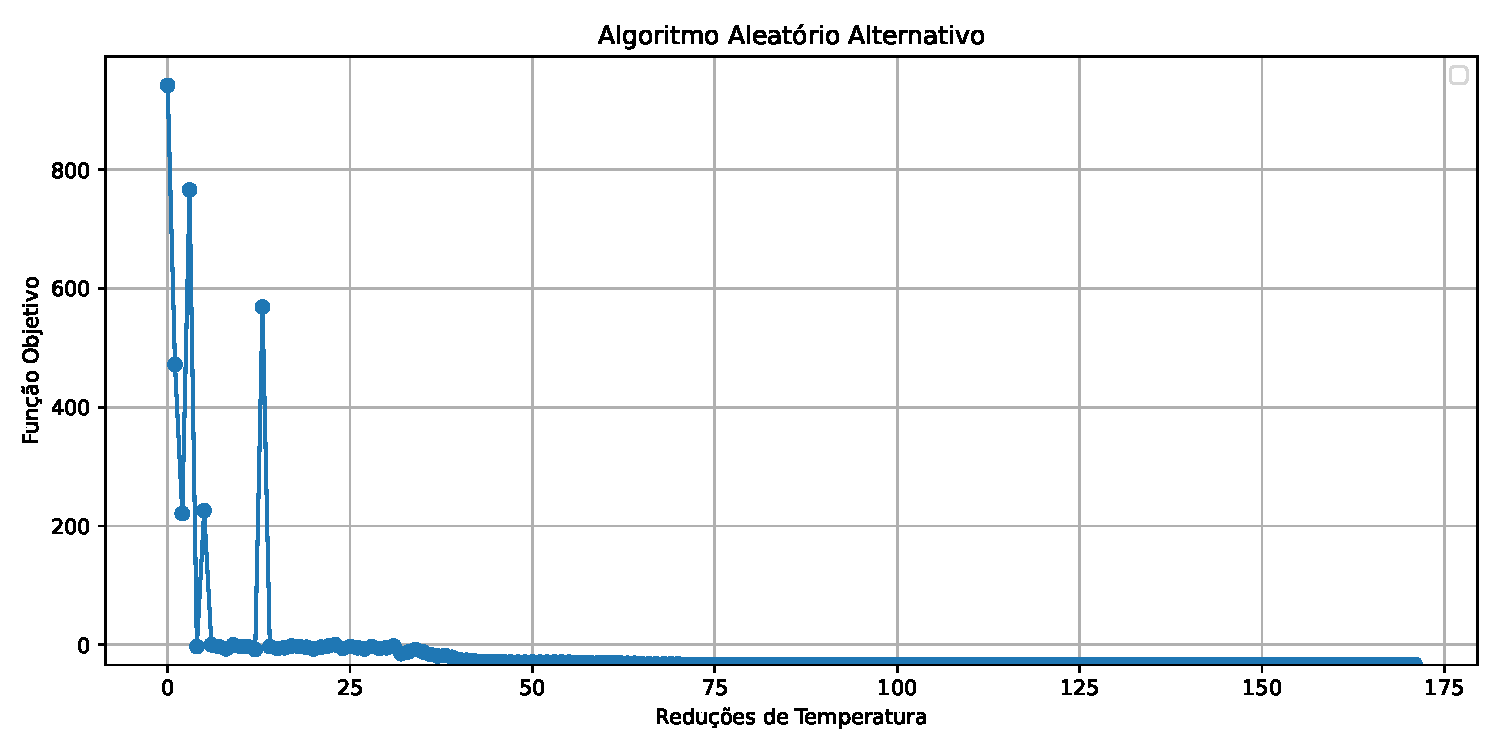
\includegraphics[width=\textwidth]{P2M1_NNGV_n_exams_random_alt}
        \caption{Função objetivo por iteração do algoritmo aleatório alt}
        \label{fig:P2M1_NNGV_n_exams_random_alt}
    \end{subfigure}
    \hfill
    \begin{subfigure}{0.49\textwidth}
        \centering
        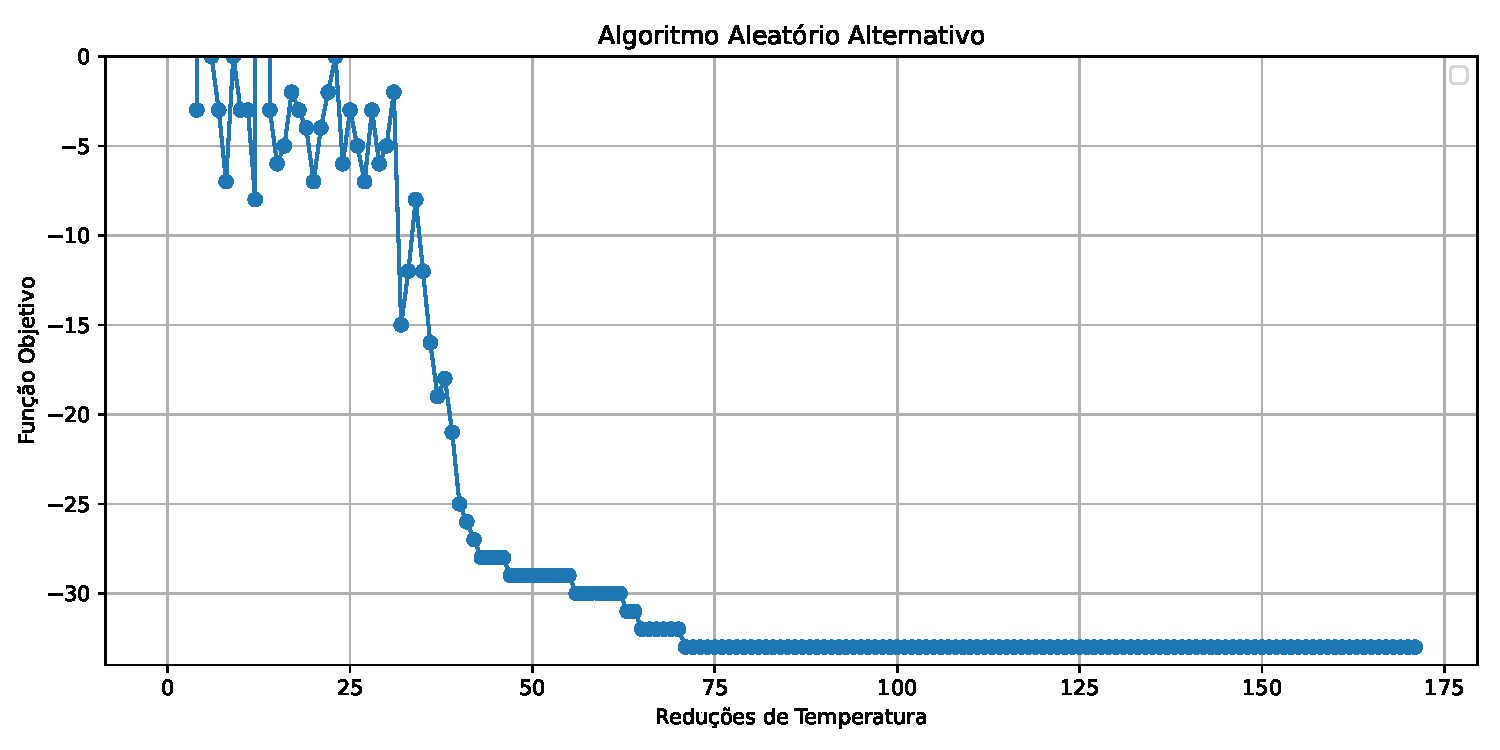
\includegraphics[width=\textwidth]{P2M1_NNGV_n_exams_random_alt_clip}
        \caption{Função objetivo por iteração do algoritmo aleatório alt limitado pelo valor máximo de 0}
        \label{fig:P2M1_NNGV_n_exams_random_alt_clip}
    \end{subfigure}
    \caption{Evolução do valor da função objetivo ao longo da otimização do problema do número de trabalhos com o Modelo 1 ($L_{k}=5000$, $CP=100$, $\alpha=0.8$, $P=10$, $p_{0}=0.9$).}
    \label{fig:P2M1_NNGV_dif_sol_ini}
\end{figure}

Foram utilizados os mesmo critérios do modelo anterior, descritos em Franzin et al.~\cite{franzinRevisitingSimulatedAnnealing2019}, ou seja, \textbf{NE1}, \textbf{UT6}, uma modificação de \textbf{SC9}, \textbf{AC1}, \textbf{CS2}, e \textbf{TL1}.\\

\subsection{Modelo 2}

Por sua vez, este modelo assegura que todos os movimentos devem assegurar a viabilidade da solução. Desta forma, a função objetivo é diferente dos modelos anteriores, ao admitir-se que a sobre-utilização de recursos não ocorre, será então dada por:
$$f(s) = \sum -Y$$

Durante a geração da vizinhança com o movimento 0 e com o movimento 2 será escolhido de forma aleatória um instante de tempo de uma lista de candidatos que não provocam sobre-utilização de recursos. Este processo é resumido à Figura~\ref{fig:P2M1_GV_gen}. Por sua vez, o Algoritmo~\ref{algo:P2M1_GV_main_algo} apresenta como se deve proceder na escolha do movimento e que passos são necessários para gerar a vizinhança, avaliá-la, aceitá-la ou rejeitá-la. O Algoritmo~\ref{algo:P2M1_GV_main_algo_rollback} apresenta como se deve fazer o retrocesso para cada movimento.\\
\begin{figure}[H]
	\centering
	\begin{subfigure}{0.49\textwidth}
	\centering
		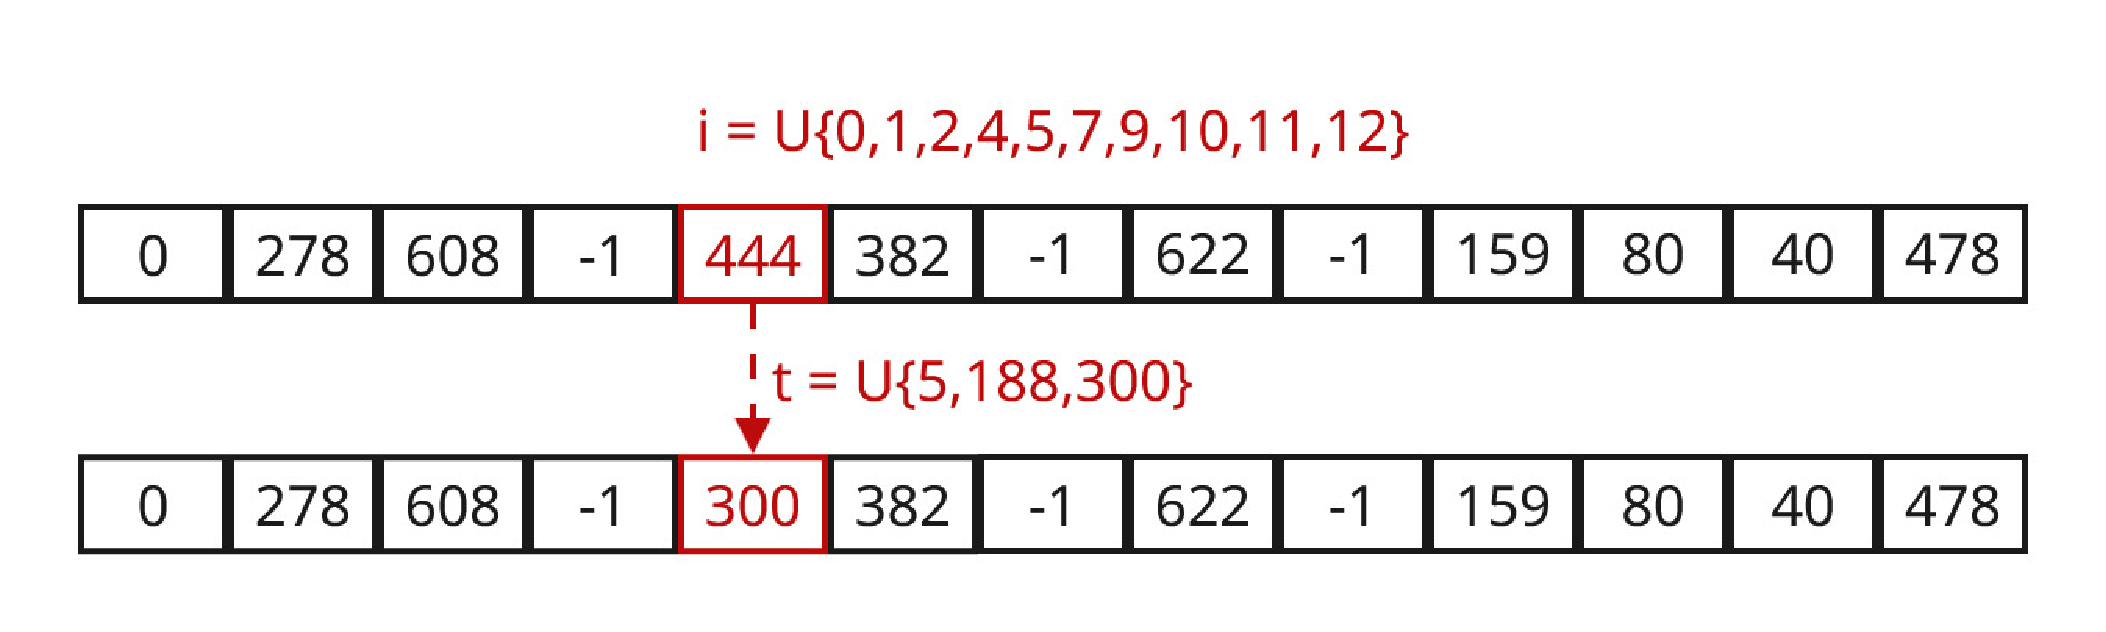
\includegraphics[width = \textwidth]{P2M1_GV_M0}
		\caption{Movimento 0}
		\label{fig:P2M1_GV_M0}
	\end{subfigure}
	\begin{subfigure}{0.49\textwidth}
	\centering
		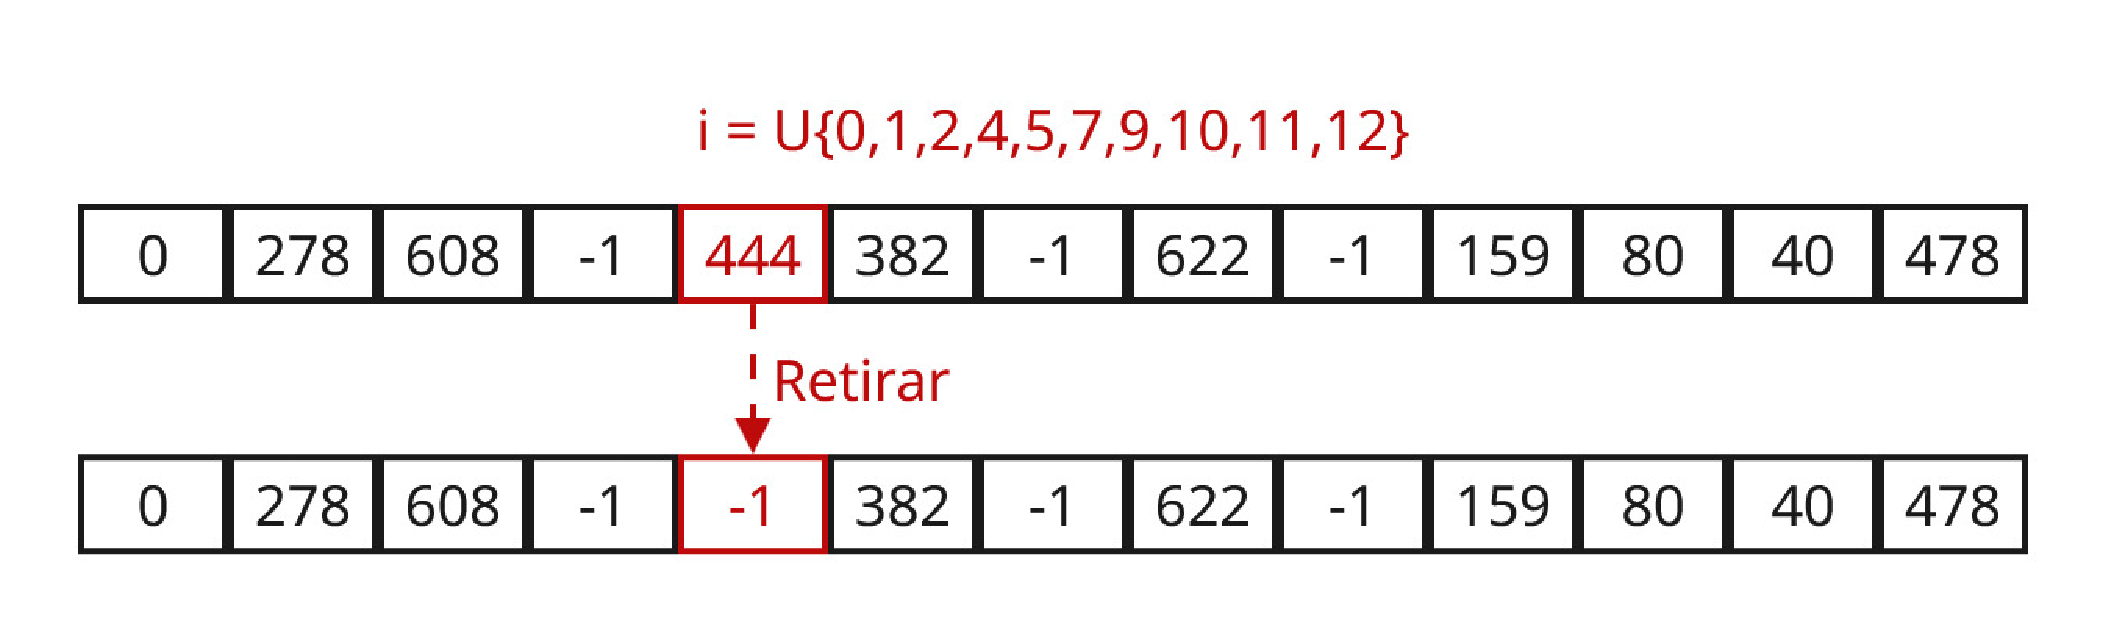
\includegraphics[width = \textwidth]{P2M1_GV_M1}
		\caption{Movimento 1}
		\label{fig:P2M1_GV_M1}
	\end{subfigure}
	\begin{subfigure}{0.49\textwidth}
	\centering
		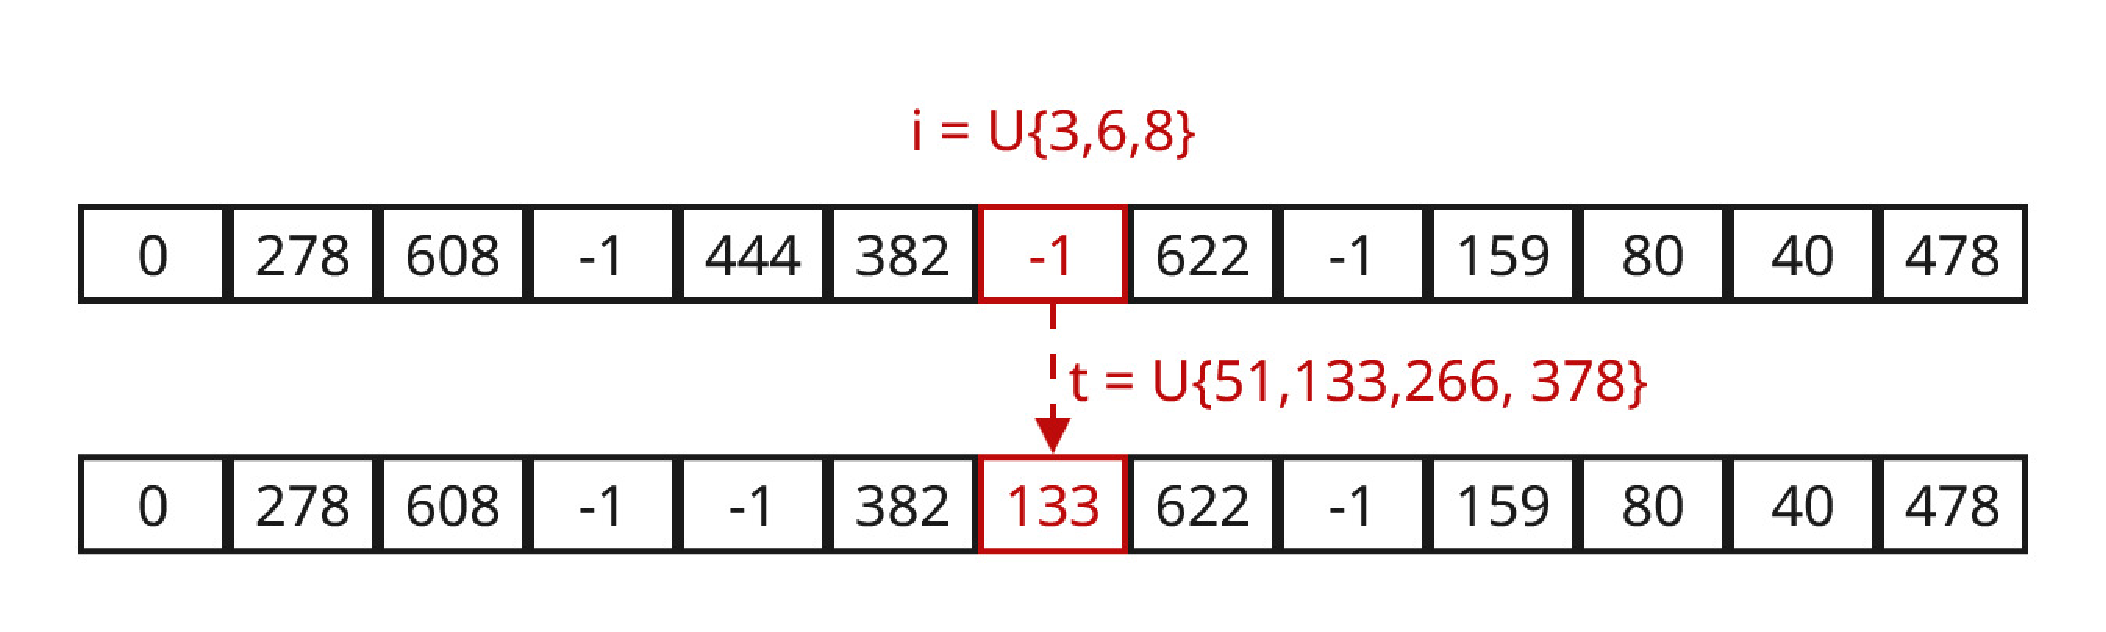
\includegraphics[width = \textwidth]{P2M1_GV_M2}
		\caption{Movimento 2}
		\label{fig:P2M1_GV_M2}
	\end{subfigure}
	\caption{Processo de transição da solução $s$ para a solução $s'$ para o modelo 3 do problema 2.}
	\label{fig:P2M1_GV_gen}
\end{figure}

A definição da temperatura inicial tem uma nuance: de forma a inflacionar a temperatura inicial não se utilizou o movimento 0, ou seja, os movimentos 1 e 2 têm 50\% de  probabilidade de ocorrem, o que aumenta o valor de $\Delta_{avg}$. Se este valor for baixo demais, nunca será considerado a remoção de um trabalho, porque o impacto sobre a função objetivo é muito grande. O modelo anterior não possui este problema devido à alta temperatura inicial, proveniente da grande variabilidade da função objetivo entre soluções.\\

A geração da solução inicial é bastante diferente em certas condições. Na Figura~\ref{fig:P2M1_GV_dif_sol_ini} encontram-se três formas de gerar a solução inicial, na Figura~\ref{fig:P2M1_GV_n_exams_random} agendam-se todos os trabalhos com instante de começo aleatório, na Figura~\ref{fig:P2M1_GV_n_exams_random_alt1} agenda-se um número aleatório de trabalhos a instantes de começo aleatórios, na Figura~\ref{fig:P2M1_GV_n_exams_random_alt2} utiliza-se o algoritmo \textit{SA} sem a inclusão do movimento 0 para gerar a solução inicial. As figuras não ilustram como se comporta função objetivo, mas sim $f(s) = \sum -Y + 10 \sum_{t=0}^{T_{\max}-1}\sum_{p}v(t,p)$, ou seja, durante o algoritmo não consideramos a sobre-utilização de recursos, mas para o gráfico é necessário reportar este elemento.\\

Ao comparar as Figuras~\ref{fig:P2M1_GV_n_exams_random},~\ref{fig:P2M1_GV_n_exams_random_alt1},~\ref{fig:P2M1_GV_n_exams_random_alt2} observa-se dois comportamentos distintos. Enquanto as Figuras~\ref{fig:P2M1_GV_n_exams_random},~\ref{fig:P2M1_GV_n_exams_random_alt1} apresentam soluções de baixa qualidade que não são capazes de superar a sobre-utilização de recursos proveniente da solução inicial, na Figura~\ref{fig:P2M1_GV_n_exams_random_alt2} é evidente que a solução inicial não apresenta qualquer sobre-utilização, permitindo que ocorra o processo normal de minimização.\\

As Figuras~\ref{fig:P2M1_GV_n_exams_random_clip},~\ref{fig:P2M1_GV_n_exams_random_alt1_clip},~\ref{fig:P2M1_GV_n_exams_random_alt2_clip} evidenciam o mesmo facto, apenas o algoritmo aleatório alternativo 2 é capaz de gerar uma solução inicial que origine soluções finais perto do ótimo.\\
\begin{figure}[H]
    \centering
    % Row 1
    \begin{subfigure}{0.49\textwidth}
        \centering
        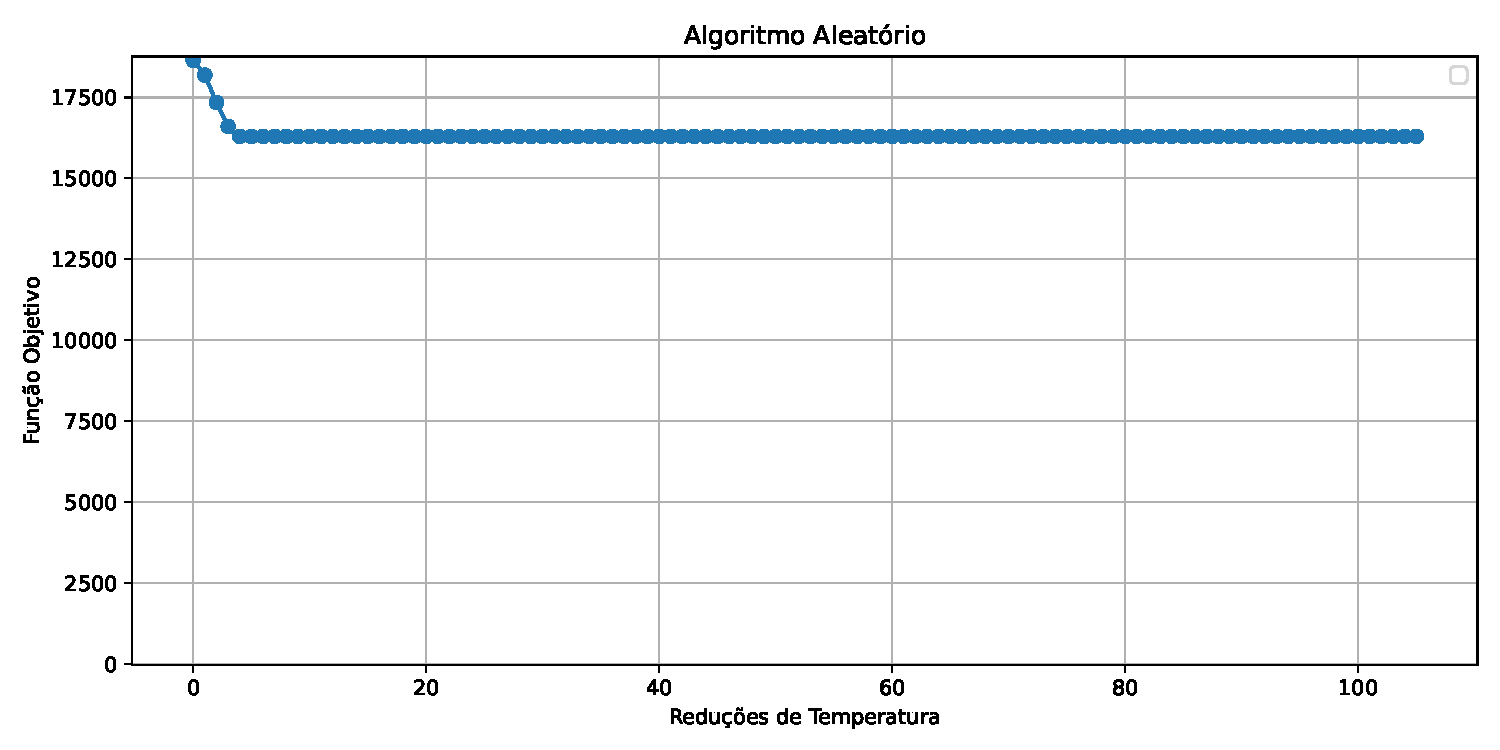
\includegraphics[width=\textwidth]{P2M1_GV_n_exams_random}
        \caption{Função objetivo por iteração do algoritmo aleatório}
        \label{fig:P2M1_GV_n_exams_random}
    \end{subfigure}
    \hfill
    \begin{subfigure}{0.49\textwidth}
        \centering
        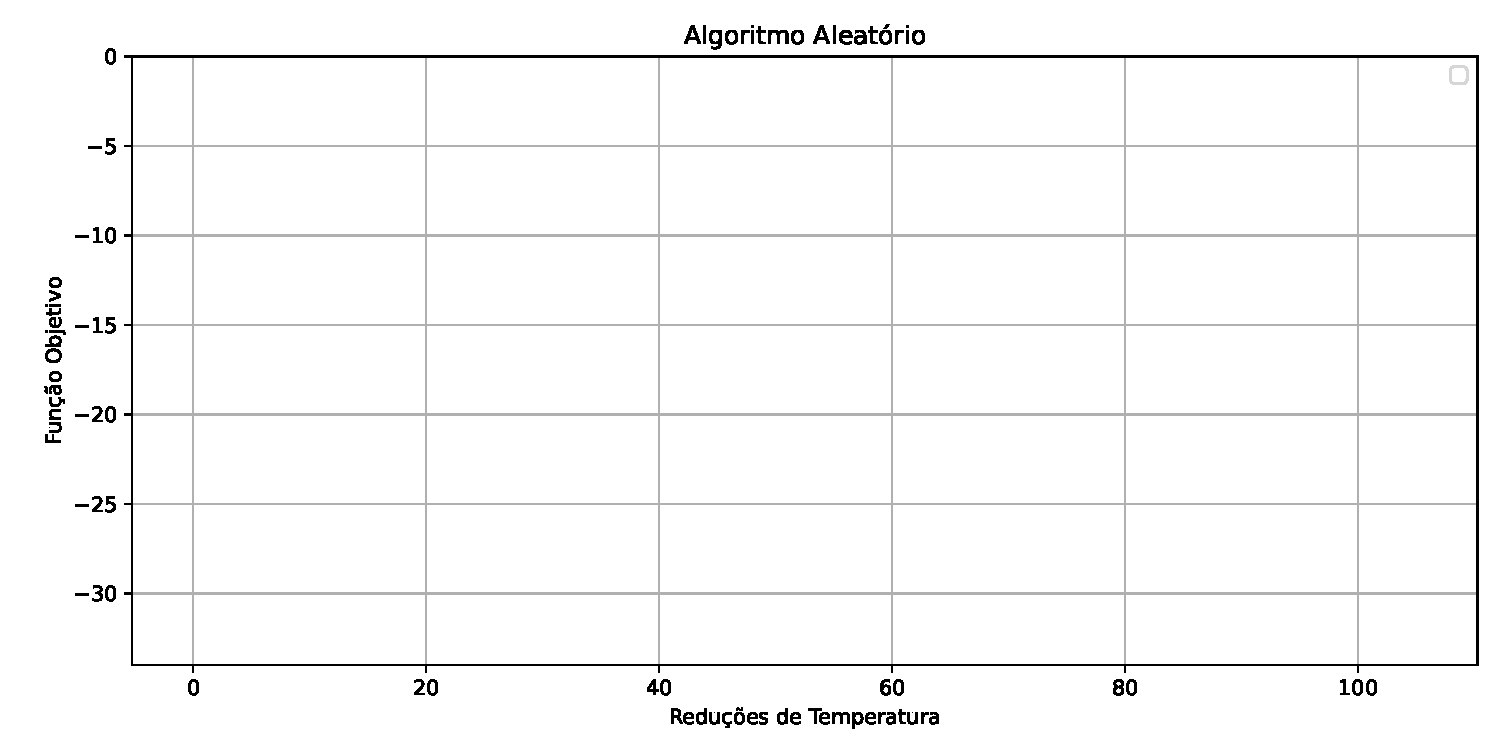
\includegraphics[width=\textwidth]{P2M1_GV_n_exams_random_clip}
        \caption{Função objetivo por iteração do algoritmo aleatório limitado pelo valor máximo de 0}
        \label{fig:P2M1_GV_n_exams_random_clip}
    \end{subfigure}
    
    % Row 2
    \begin{subfigure}{0.49\textwidth}
        \centering
        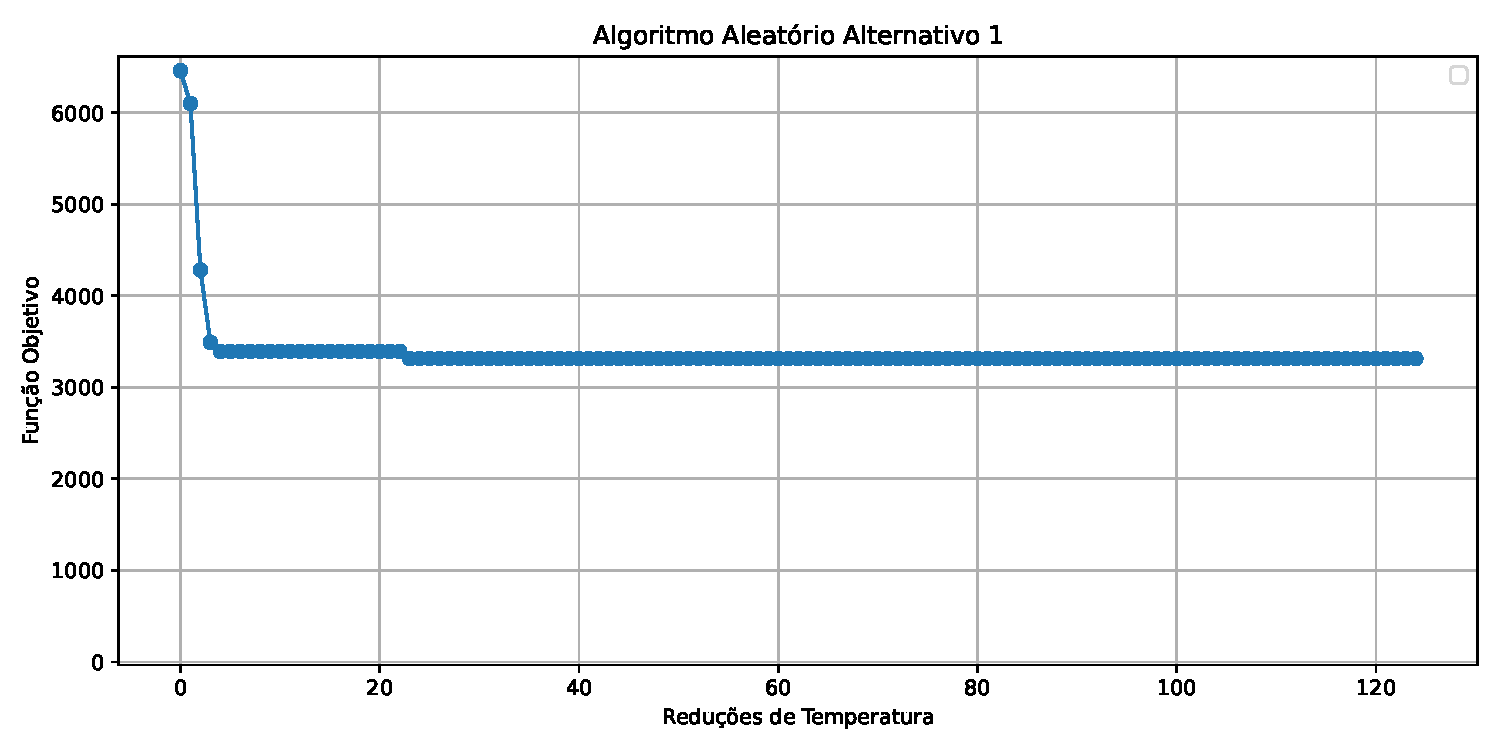
\includegraphics[width=\textwidth]{P2M1_GV_n_exams_random_alt1}
        \caption{Função objetivo por iteração do algoritmo aleatório alt 1}
        \label{fig:P2M1_GV_n_exams_random_alt1}
    \end{subfigure}
    \hfill
    \begin{subfigure}{0.49\textwidth}
        \centering
        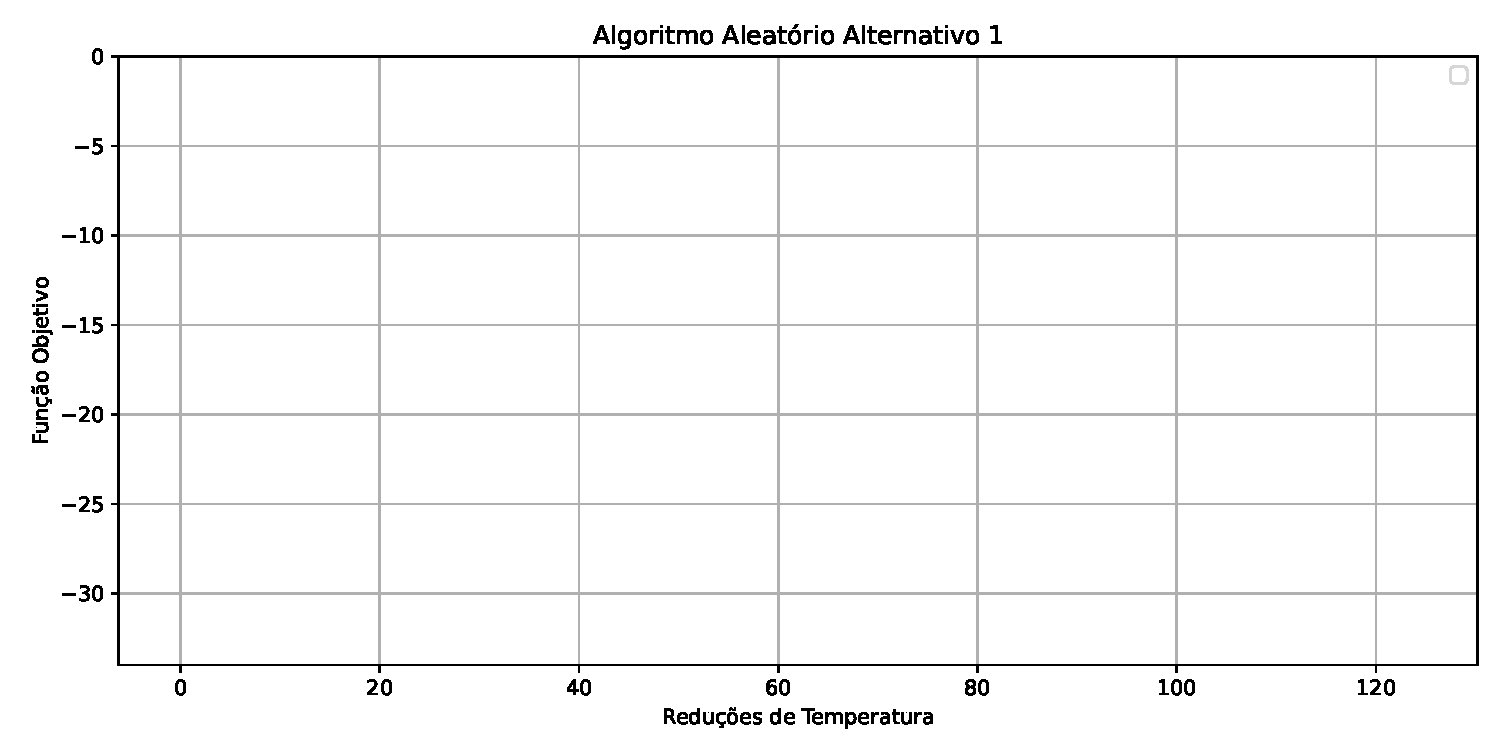
\includegraphics[width=\textwidth]{P2M1_GV_n_exams_random_alt1_clip}
        \caption{Função objetivo por iteração do algoritmo aleatório alt 1 limitado pelo valor máximo de 0}
        \label{fig:P2M1_GV_n_exams_random_alt1_clip}
    \end{subfigure}
    
    % Row 3
    \begin{subfigure}{0.49\textwidth}
        \centering
        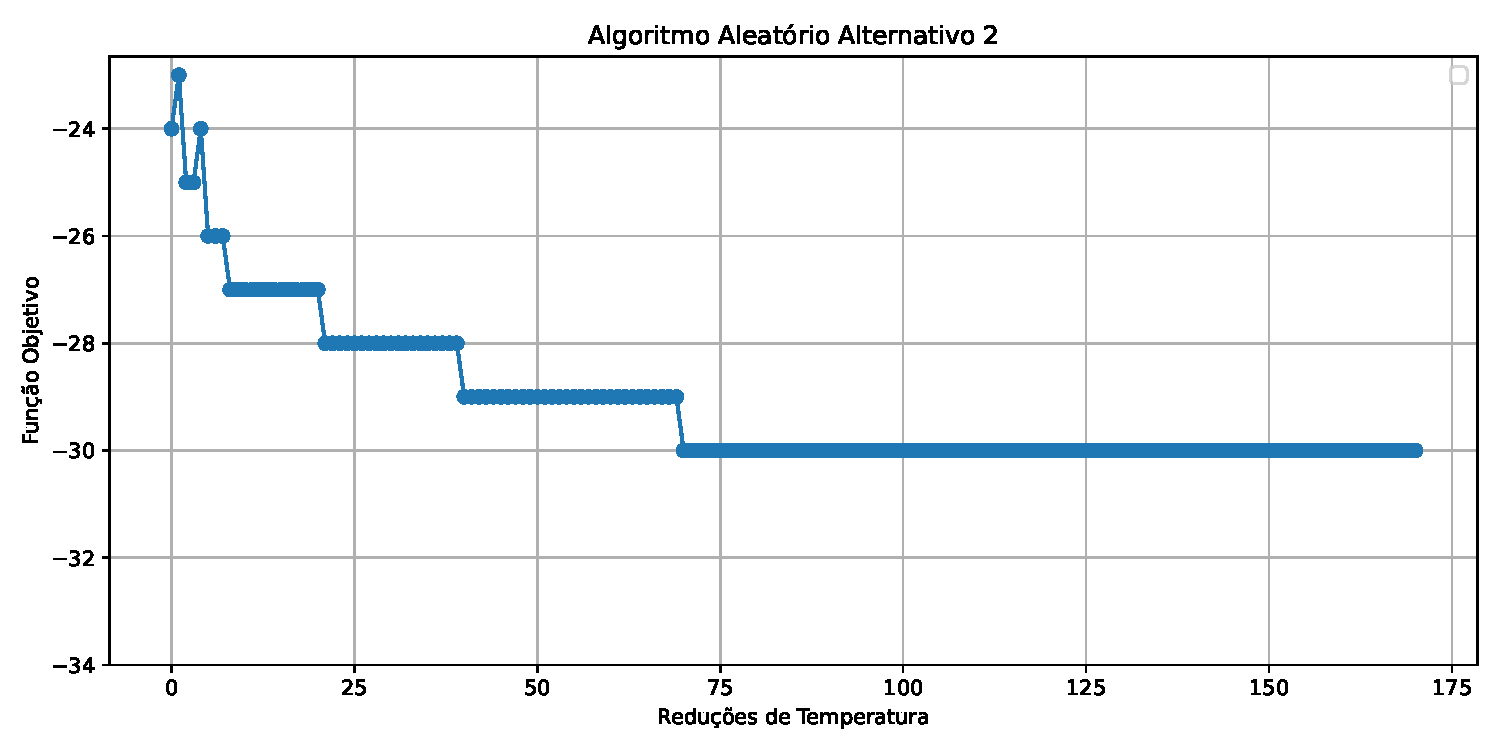
\includegraphics[width=\textwidth]{P2M1_GV_n_exams_random_alt2}
        \caption{Função objetivo por iteração do algoritmo aleatório alt 2}
        \label{fig:P2M1_GV_n_exams_random_alt2}
    \end{subfigure}
    \hfill
    \begin{subfigure}{0.49\textwidth}
        \centering
        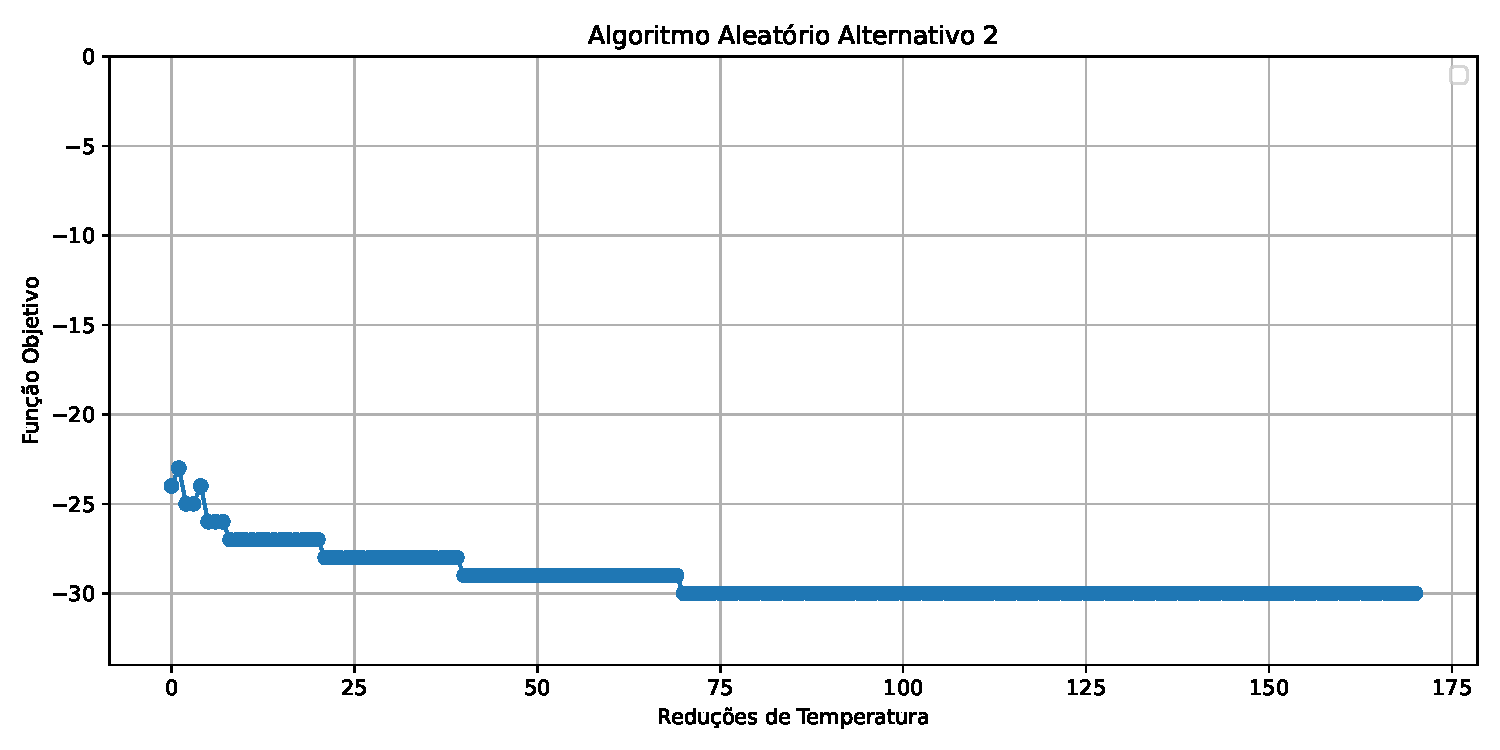
\includegraphics[width=\textwidth]{P2M1_GV_n_exams_random_alt2_clip}
        \caption{Função objetivo por iteração do algoritmo aleatório alt 2 limitado pelo valor máximo de 0}
        \label{fig:P2M1_GV_n_exams_random_alt2_clip}
    \end{subfigure}
    \caption{Evolução do valor da função objetivo ao longo da otimização do problema do número de trabalhos com o Modelo 2 ($L_{k}=100$, $CP=100$, $\alpha=0.8$, $P=0$, $p_{0}=0.5$).}
    \label{fig:P2M1_GV_dif_sol_ini}
\end{figure}

A diferença demonstrada entre os três algoritmos deve-se a uma combinação entre baixa temperatura inicial, um valor baixo de $L_{k}$ e a assumida inexistência de punição $P$, com o aumento de um destes parâmetros observa-se que a diferença entre os algoritmo é irrelevante. A baixa temperatura torna difícil a remoção de trabalhos mesmo ao causarem sobre-utilização de recursos, o valor baixo de $L_{k}$ restringe o número de vizinhos visitados no início da procura, e a inexistência de punição não permite direcionar o algoritmo para que se remova exames que causam sobre-utilização.\\
Desta forma irá ser utilizado o algoritmo de geração da solução inicial proveniente da Figura~\ref{fig:P2M1_GV_n_exams_random_alt2}, sendo esta a mais robusta, funcionando para qualquer combinação de níveis.\\

Foram utilizados os mesmo critérios do modelo anterior, descritos em Franzin et al.~\cite{franzinRevisitingSimulatedAnnealing2019}, ou seja, \textbf{NE1}, \textbf{UT6}, uma modificação de \textbf{SC9}, \textbf{AC1}, \textbf{CS2}, e \textbf{TL1}.\\

\subsection{Modelo 3}

Este modelo já utiliza uma codificação diferente, utilizado a sequência de agendamento como solução. Ao mesmo tempo, ao contrário dos modelos já descritos, não é necessário existirem vários movimentos, sendo apenas considerado a alteração da sequência. Como já previamente discutido, a alteração da sequência pode ocorrer de várias formas, pela troca de índices, pela inserção de um trabalho noutro índice, ou pela inversão de sub-sequências, mas apenas o primeiro método foi considerado.\\
Por sua vez, a função objetivo não é diretamente derivada pela solução. Sendo primeiro necessário utilizar um algoritmo de \textit{timetabling} para descodificar a solução. Mesmo assim, a função objetivo é dada por:
$$f(s) = \sum -Y$$

Para a obtenção da variável $Y$ verifica-se que trabalhos acabam antes do tempo pré-definido, $T_{\max}$. Por isso, durante o algoritmo de \textit{timetabling} pode-se realizar o agendamento como no problema de \textit{makespan}, ou seja, tentando agendar cada trabalho o mais cedo possível. Outra possibilidade será agendar o mais cedo possível cada trabalho, mas agendar o mais tarde possível aqueles trabalhos que acabariam depois de $T_{\max}$. A Figura~\ref{fig:P2M2_GV_tt} pretende demonstrar esta diferença.\\
\begin{figure}[H]
	\centering
	\begin{subfigure}{0.49\textwidth}
	\centering
		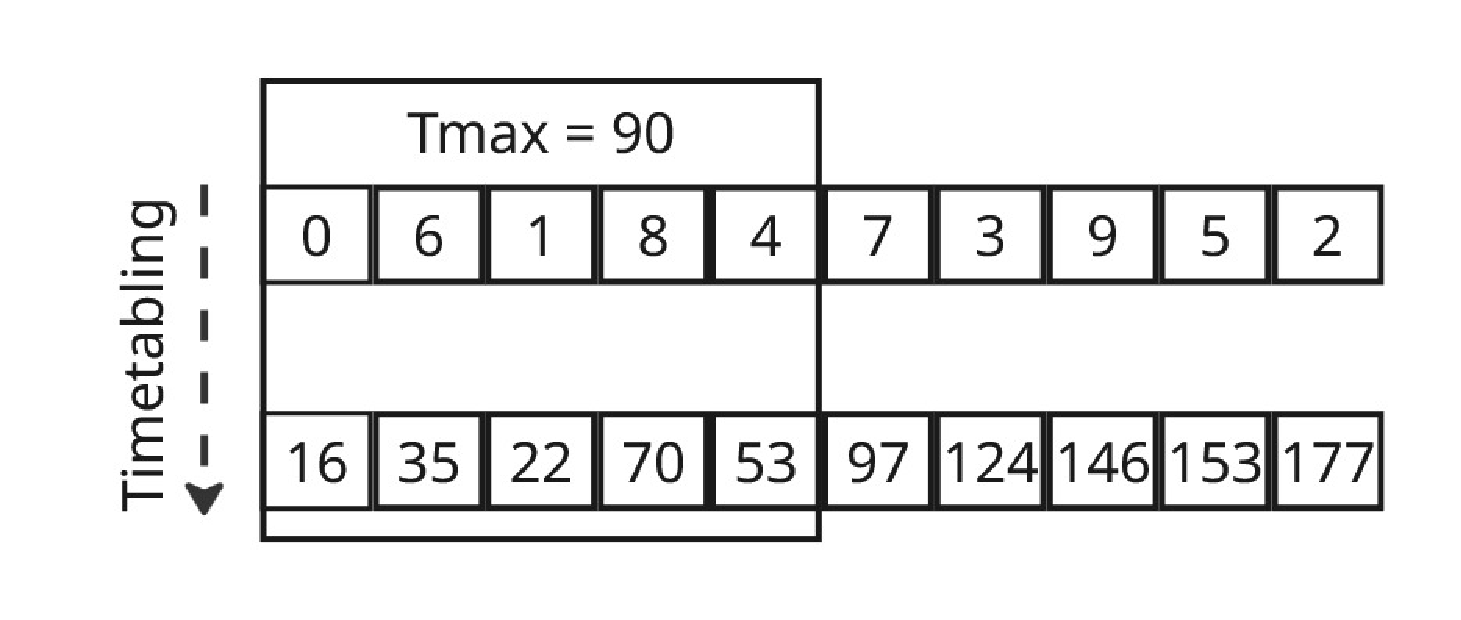
\includegraphics[width = \textwidth]{P2M2_GV_tt1}
		\caption{\textit{Timetabling} como no problema de \textit{makespan}}
		\label{fig:P2M2_GV_tt1}
	\end{subfigure}
	\begin{subfigure}{0.49\textwidth}
	\centering
		\includegraphics[width = \textwidth]{P2M2_GV_tt2}
		\caption{\textit{Timetabling} modificado}
		\label{fig:P2M2_GV_tt2}
	\end{subfigure}
	\caption{As duas possibilidades para o algoritmo de \textit{timetabling}.}
	\label{fig:P2M2_GV_tt}
\end{figure}

Neste exemplo ilustrativo evidencia-se a diferença entre as duas possibilidade. Na Figura~\ref{fig:P2M2_GV_tt1}, durante o agendamento do trabalho 7 este não permite que o trabalho 3 comece mais cedo. Quando comparado com a Figura~\ref{fig:P2M2_GV_tt2}, ao agendar o trabalho 7 para o instante $T_{\max}$ permite-se agendar o trabalho 3 num instante que vai ser englobado na solução, o que melhora a qualidade da solução com a mesma agenda. O Algoritmo~\ref{algo:left-shift-TT_P2} apresenta o pseudo-código que define a diferença.\\
 
Como podem existir vários trabalhos iguais, deve-se assegurar que durante a geração da vizinhança não se considera a troca de dois trabalhos do mesmo tipo, de forma a evitar gerar uma nova solução igual à atual. Ao mesmo tempo existem trocas que parecem ser desnecessárias, este facto apresenta-se na figura~\ref{fig:P2M2_GV_troca}.\\
\begin{figure}[H]
	\centering
	\begin{subfigure}{0.49\textwidth}
	\centering
		\includegraphics[width = \textwidth]{P2M2_GV_troca1}
		\caption{Troca de dois trabalhos pertencentes à \\solução}
		\label{fig:P2M2_GV_troca1}
	\end{subfigure}
	\begin{subfigure}{0.49\textwidth}
	\centering
		\includegraphics[width = \textwidth]{P2M2_GV_troca2}
		\caption{Troca de um trabalho pertencente à solução e de um não pertencente}
		\label{fig:P2M2_GV_troca2}
	\end{subfigure}
	\begin{subfigure}{0.49\textwidth}
	\centering
		\includegraphics[width = \textwidth]{P2M2_GV_troca3}
		\caption{Troca de dois trabalhos não pertencentes à solução}
		\label{fig:P2M2_GV_troca3}
	\end{subfigure}
	\caption{As três trocas que podem ocorrer.}
	\label{fig:P2M2_GV_troca}
\end{figure}

Evidencia-se o porquê de algumas das trocas possíveis não serem interessantes no processo de otimização. Para as trocas representadas pelas Figuras~\ref{fig:P2M2_GV_troca1},~\ref{fig:P2M2_GV_troca2} prevê-se que a solução seja diferente da a atual, mesmo que o número de trabalhos que acabem antes de $T_{\max}$ não se altere, os instantes de começo para estes exames são diferentes. Por outro lado, a troca apresentada na Figura~\ref{fig:P2M2_GV_troca3} não deve ter impacto sobre os instantes de começo dos trabalhos que acabem antes de $T_{\max}$. Contudo, não se vai influenciar como ocorrem as trocas representadas pela Figura~\ref{fig:P2M2_GV_troca}, isto porque é computacionalmente dispendioso verificar que trocas entre trabalhos, que acabam depois de $T_{\max}$, de facto têm influencia sobre a solução. O Algoritmo~\ref{algo:P2M2_GV_main_algo} apresenta o processo de geração da vizinhança, de avaliação, rejeição ou aceitação, atribuição da melhor solução, e possível retrocesso.\\

No modelo análogo do problema anterior utilizou-se \textit{left-shift timetabling} para descodificar a solução, e o mesmo foi feito aqui. Propôs-se também a utilização de \textit{enchanced left-shift timetabling}, para o problema anterior esta alternativa melhorava a qualidade da solução em troco de maior tempo computacional. Como a sequência inversa engloba um conjunto diferente de trabalhos que acabam antes de $T_{\max}$ não há relação entre a agenda \textit{forward} e \textit{backward}, a Figura~\ref{fig:P2M2_GV_tt_for_back} pretende demonstrar este facto.\\
\begin{figure}[H]
	\centering
	\begin{subfigure}{0.49\textwidth}
	\centering
		\includegraphics[width = \textwidth]{P2M2_GV_tt2}
		\caption{Agenda \textit{forward}}
		\label{fig:P2M2_GV_tt2}
	\end{subfigure}
	\begin{subfigure}{0.49\textwidth}
	\centering
		\includegraphics[width = \textwidth]{P2M2_GV_tt2_backwards}
		\caption{Agenda \textit{backward}}
		\label{fig:P2M2_GV_tt2_backwards}
	\end{subfigure}
	\caption{Agenda ilustrativa utilizando \textit{enhanced left-shifting}.}
	\label{fig:P2M2_GV_tt_for_back}
\end{figure}

A temperatura inicial será definida com a geração de uma boa solução pela heurística NEH, de seguida será realizada a caminhada aleatória com $c=\infty$ e $L_{k}=1000$ e com a temperatura inicial calculada por $c_{0}=|\Delta_{avg}/log(p_{0})|$. O valor de $\Delta_{avg}$ é baixo, contudo isto não causa um problema tão grande como no modelo anterior, porque não ocorre explicitamente a remoção de trabalhos da solução.\\

Não existem muitas opções para a geração da solução inicial, por isso gerou-se uma sequência aleatória para tal, delimitada na Figura~\ref{fig:P2M2_GV_dif_sol_ini}. Na figura~\ref{fig:P2M2_GV_n_exams_random},~\ref{fig:P2M2_GV_n_exams_random_clip} a evolução da função objetivo ao longo do algoritmo segue o já observado, um aumento da função objetivo seguido da sua diminuição e por fim aciona-se o critério de paragem $CP$. \\
\begin{figure}[H]
    \centering
    % Row 1
    \begin{subfigure}{0.49\textwidth}
        \centering
        \includegraphics[width=\textwidth]{P2M2_GV_n_exams_random}
        \caption{Função objetivo por iteração do algoritmo aleatório}
        \label{fig:P2M2_GV_n_exams_random}
    \end{subfigure}
    \hfill
    \begin{subfigure}{0.49\textwidth}
        \centering
        \includegraphics[width=\textwidth]{P2M2_GV_n_exams_random_clip}
        \caption{Função objetivo por iteração do algoritmo aleatório limitado pelo valor máximo de 0}
        \label{fig:P2M2_GV_n_exams_random_clip}
    \end{subfigure}
    \caption{Evolução do valor da função objetivo ao longo da otimização do problema do número de trabalhos com o Modelo 3 ($L_{k}=500$, $CP=100$, $\alpha=0.8$, $P=10$, $p_{0}=0.9$, \textit{left-shift timetabling}, geração de vizinhos através de troca).}
    \label{fig:P2M2_GV_dif_sol_ini}
\end{figure}

Foram utilizados os mesmo critérios do modelo anterior, descritos em Franzin et al.~\cite{franzinRevisitingSimulatedAnnealing2019}, ou seja, \textbf{NE1}, \textbf{UT6}, uma modificação de \textbf{SC9}, \textbf{AC1}, \textbf{CS2}, e \textbf{TL1}.\\